%% ====================================================================
%%  AEGIS: Adaptive Execution Guarded Interpreter System
%%  IEEE Conference Paper — Full Submission Version
%%  Format: IEEEtran, conference, two-column, US Letter
%% ====================================================================
\documentclass[conference]{IEEEtran}
\IEEEoverridecommandlockouts

%% ---- Packages -------------------------------------------------------
\usepackage{cite}
\usepackage{amsmath,amssymb,amsfonts}
\usepackage{graphicx}
\usepackage{textcomp}
\usepackage{xcolor}
\usepackage{booktabs}
\usepackage{multirow}
\usepackage{array}
\usepackage{tabularx}
\usepackage{url}
\usepackage{balance}
\usepackage{microtype}
\usepackage{listings}
\usepackage{tikz}
\usetikzlibrary{
  shapes.geometric, arrows.meta, positioning, fit,
  decorations.pathreplacing, backgrounds, calc,
  arrows, shapes.multipart, patterns
}
\usepackage{algorithm}
\usepackage{algpseudocode}
\renewcommand{\algorithmicrequire}{\textbf{Input:}}
\renewcommand{\algorithmicensure}{\textbf{Output:}}
\usepackage{pgfplots}
\pgfplotsset{compat=1.18}
\usepackage{subcaption}
\usepackage{enumitem}

%% ---- TikZ Styles ---------------------------------------------------
\tikzset{
  %% Generic rounded rectangle
  rbox/.style={
    rectangle, rounded corners=4pt,
    draw=#1!65!black, fill=#1!10,
    text centered, font=\scriptsize,
    inner sep=4pt, minimum height=0.6cm,
    line width=0.55pt
  },
  rbox/.default=blue,
  %% Arrow
  arr/.style={-{Stealth[length=5pt,width=4pt]},
              draw=black!65, line width=0.8pt},
  darr/.style={{Stealth[length=4pt,width=3.5pt]}-%
               {Stealth[length=4pt,width=3.5pt]},
               draw=black!55, line width=0.8pt},
  %% Stage box in pipeline
  stage/.style={
    rectangle, rounded corners=3pt,
    draw=#1!70!black, fill=#1!12,
    minimum width=3.5cm, minimum height=0.58cm,
    text centered, font=\scriptsize\bfseries,
    inner sep=3pt, line width=0.6pt
  },
  stage/.default=teal,
  %% Defense layer
  dlayer/.style={
    rectangle, rounded corners=2pt,
    draw=black!55, fill=#1!18,
    minimum height=0.5cm,
    text centered, font=\scriptsize\bfseries,
    inner sep=3pt, line width=0.5pt
  },
  dlayer/.default=blue,
  %% Diamond decision
  diam/.style={
    diamond, draw=orange!70!black, fill=orange!12,
    text centered, font=\tiny\bfseries,
    aspect=3, minimum height=0.42cm,
    inner sep=1.5pt, line width=0.6pt
  },
}

%% ---- Listings Style ------------------------------------------------
\lstset{
  basicstyle   = \ttfamily\scriptsize,
  breaklines   = true,
  frame        = single,
  rulecolor    = \color{black!35},
  backgroundcolor = \color{gray!6},
  keywordstyle = \color{blue!70}\bfseries,
  commentstyle = \color{green!50!black}\itshape,
  stringstyle  = \color{orange!75!black},
  numbers      = none,
  xleftmargin  = 5pt,
  xrightmargin = 5pt,
  aboveskip    = 4pt,
  belowskip    = 4pt,
}

%% ====================================================================
\begin{document}
%% ====================================================================

%% ---- Title ---------------------------------------------------------
\title{AEGIS: Adaptive Execution Guarded Interpreter System ---
A Security-First Framework for Trust-Based Dynamic Code Execution}

%% ---- Authors -------------------------------------------------------
\author{

\small

\begin{tabular}{ccc}

\begin{tabular}{c}
\textbf{Shweta Tiwaskar}\\
\textit{Dept. of Computer Engineering}\\
Vishwakarma Institute of Technology\\
Pune, India\\
shweta.tiwaskar@vit.edu
\end{tabular}

&

\begin{tabular}{c}
\textbf{Adarsh Jayfale}\\
\textit{Dept. of Computer Engineering}\\
Vishwakarma Institute of Technology\\
Pune, India\\
adarsh.jayfale24@vit.edu
\end{tabular}

&

\begin{tabular}{c}
\textbf{Wasim Pathan}\\
\textit{Dept. of Computer Engineering}\\
Vishwakarma Institute of Technology\\
Pune, India\\
wasim.pathan24@vit.edu
\end{tabular}

\\[1.1cm]

\multicolumn{3}{c}{

\begin{tabular}{cc}

\begin{tabular}{c}
\textbf{Nilesh Sabale}\\
\textit{Dept. of Computer Engineering}\\
Vishwakarma Institute of Technology\\
Pune, India\\
nilesh.sabale24@vit.edu
\end{tabular}

& \hspace{1.5cm}

\begin{tabular}{c}
\textbf{Adesh Bhore}\\
\textit{Dept. of Computer Engineering}\\
Vishwakarma Institute of Technology\\
Pune, India\\
adesh.bhore24@vit.edu
\end{tabular}

\end{tabular}

}

\end{tabular}

}

\maketitle

%% ====================================================================
%%  ABSTRACT
%% ====================================================================
\begin{abstract}
Running code from untrusted sources safely remains one of the
harder open problems in cloud platforms, online judges, and
multi-tenant computing environments. The mainstream
approaches---hardware sandboxes, static analysis, and blanket
trust---each solve part of the problem while leaving significant
gaps in security coverage, execution speed, or the ability to
adapt to a program's observed behavior. We present
\textbf{AEGIS} (\textbf{A}daptive \textbf{E}xecution
\textbf{G}uarded \textbf{I}nterpreter \textbf{S}ystem), an
interpreter framework built around a \emph{trust-based adaptive
execution model} that bridges these gaps without permanently
sacrificing either isolation or throughput. Under AEGIS, every
program starts in a tightly constrained sandbox. A quantitative
\emph{TrustScore}, rooted in accumulated evidence of safe
behavior across multiple runs, governs whether a program earns
promotion to an AST-optimized fast path. The moment any runtime
violation surfaces, the system rolls back: the cached optimized
AST is discarded, the trust score drops to zero, and the program
returns to full sandbox enforcement. Internally, AEGIS operates
as a seven-stage pipeline---lexical analysis, parsing,
conservative static security screening, trust-gated mode
selection, dual-path execution, runtime monitoring, and rollback
handling---served through a REST\,API and a Monaco-based web IDE.
We evaluated the framework on arithmetic-heavy, control-flow-heavy,
and adversarial benchmarks. Trust-promoted code runs
\textbf{2.52$\times$} faster on average, the combined
static-plus-runtime analysis catches \textbf{every planted
vulnerability} across one hundred handcrafted test programs, and
rollback completes in a mean of \textbf{1.84\,ms}---well below
interactive latency thresholds. These results indicate that
treating demonstrated safety as a first-class optimization signal
offers a practical path toward reconciling the tension between
strong isolation and competitive performance in untrusted-code
execution settings.
\end{abstract}

\begin{IEEEkeywords}
interpreter security, adaptive execution, trust management,
sandboxed execution, static analysis, runtime monitoring, rollback,
AST optimization, code cache, security-first design
\end{IEEEkeywords}

%% ====================================================================
\section{Introduction}
%% ====================================================================

The need to run code from untrusted sources is nearly
ubiquitous in modern computing.  Online judges evaluate student
submissions, browser-based IDEs let strangers edit and execute
programs on shared servers, and serverless platforms routinely
invoke user-supplied functions inside multi-tenant
clusters~\cite{johnson2023wave,menetrey2024sgx,li2022iot_trust}.
What all these settings share is a fundamental tension:
the host must protect itself from malicious or buggy inputs
while keeping execution fast enough that legitimate users
do not notice the safety net.

Three broad families of defense have emerged to address this
tension, and each one leaves something on the table.
\emph{Hardware-assisted sandboxing}, as realized by WebAssembly
runtimes and Intel SGX enclaves, delivers strong isolation
guarantees but pays for them with bounds-checking overhead,
restricted system-call surfaces, and sometimes complex
deployment~\cite{johnson2023wave,menetrey2024sgx}.
\emph{Static analysis} can flag certain classes of defects
before a single instruction runs, yet Rice's theorem ensures
that no sound analyzer is also complete; practitioners
consistently report that missed vulnerabilities---false
negatives---are the more dangerous failure
mode~\cite{ami2024false_neg,huang2024static}.
\emph{Implicit trust}, where submissions execute without any
gatekeeping, maximizes throughput at the expense of exposing
the platform to every attack the submitted program
carries~\cite{ullah2024deeptrust}.

A useful observation is that code in interactive environments
is rarely executed once.  Students resubmit, developers iterate,
and automated pipelines re-run the same logic many times.  Each
clean execution is a piece of evidence that the program falls
within acceptable bounds.  If a system could accumulate and act
on that evidence, it could relax costly protections for programs
that have repeatedly proved harmless, while maintaining full
enforcement for everything else.  This is the central idea
behind AEGIS.

Compiler theory offers a natural scaffolding for this kind of
staged enforcement.  The classical pipeline---lexical analysis,
parsing, semantic analysis, IR generation, optimization, code
emission~\cite{aho2007compilers}---already partitions processing
into well-defined phases, each of which can double as a
validation checkpoint.  Lexical analysis rejects malformed
tokens, parsing enforces grammatical correctness, and semantic
analysis catches type errors and undefined names.  Extending
this progression with security-specific phases (threat-aware
static checking, trust evaluation, runtime monitoring) yields
defense-in-depth without discarding the modularity that makes
compilers tractable to build and reason about.

Interpreters sit at the other end of the compilation spectrum
and happen to be the execution model of choice for the very
environments where untrusted code appears most often.  By
walking the AST or a bytecode representation directly, an
interpreter can instrument every single operation with bounds
checks and resource limits, all while preserving the
sub-second feedback loops that interactive platforms
demand~\cite{aho2007compilers}.

Relying on static techniques alone to secure these environments,
however, is provably incomplete.  Empirical studies show that
even mature, industry-grade analyzers regularly miss
vulnerabilities whose manifestation depends on runtime data
flows and complex aliasing
patterns~\cite{ami2024false_neg,huang2024static}.  This gap
between what static tools \emph{promise} and what they
\emph{deliver} motivates pairing pre-execution analysis with
dynamic monitoring so that the two layers compensate for each
other's blind spots.

The question, then, is how to design a system that starts
conservative and gradually learns to relax.  A uniform security
posture treats every invocation identically, penalizing programs
that have already proved safe with overhead they do not need.
A permissive default grants full privileges to everyone,
leaving the platform exposed to the first adversarial
submission.  What is needed is a middle path: an execution
framework that enforces strict isolation by default but awards
performance to programs that \emph{earn} it through repeated
clean runs---and revokes that award the instant a violation
appears.

Trust management models, widely deployed in distributed systems
and IoT networks to govern resource access based on behavioral
history~\cite{wang2022trust,li2022iot_trust,ullah2024deeptrust},
supply exactly this pattern.  AEGIS re-purposes the concept for
a different access right: the privilege of running on a faster,
less-restricted execution path inside a single-node interpreter.

Concretely, AEGIS realizes this vision through a seven-stage
pipeline modeled after classical compiler architecture but
augmented with security gates.  The first three stages---lexical
analysis, parsing, and conservative static
checking~\cite{aho2007compilers}---are standard.  The fourth
stage, \emph{trust evaluation}, is novel: it inspects a
persistent, SHA-256-keyed score that records the program's
execution history and decides whether to route the program to
a sandboxed interpreter or to an AST-optimized executor.
After execution, a runtime monitor validates resource limits
and security invariants; the trust store is updated; and,
if necessary, a rollback handler atomically revokes the
program's earned privileges.

\subsection*{Contributions}
The principal contributions of this work are:
\begin{enumerate}
  \item \textbf{Trust-based adaptive execution model:} a formal,
    quantitative TrustScore mechanism that controls mode promotion
    from sandboxed interpretation to AST-optimized execution, using
    security evidence rather than profiling signals
    (Section~\ref{sec:trust}).
  \item \textbf{Seven-stage auditable pipeline:} a modular execution
    pipeline with per-stage telemetry, conservative static security
    analysis, dual execution engines, and persistent trust bookkeeping
    across sessions (Section~\ref{sec:arch}).
  \item \textbf{Defense-in-depth security model:} five concentric
    enforcement layers addressing lexical, syntactic, semantic,
    runtime, and trust-gate threat surfaces, with five formally
    stated security guarantees (Section~\ref{sec:security}).
  \item \textbf{Sub-millisecond rollback:} a rollback handler that
    invalidates cache, resets trust, and reverts execution mode upon
    violation detection within a mean latency of 1.84\,ms
    (Sections~\ref{sec:trust} and~\ref{sec:eval}).
  \item \textbf{Full-stack implementation and evaluation:} a Python
    core interpreter ($\sim$5,500 LOC), Flask REST\,API, and React
    IDE ($\sim$16,000 total LOC), evaluated against performance,
    detection accuracy, trust
    dynamics, and rollback latency benchmarks
    (Sections~\ref{sec:impl} and~\ref{sec:eval}).
\end{enumerate}

\subsection*{Flow of Papers Under Contribution}

The design rationale for AEGIS emerges from a clear chain of
observations drawn from the prior literature. First, work on
hardware-assisted sandboxing~\cite{johnson2023wave,menetrey2024sgx}
establishes that strong isolation is achievable but imposes fixed
overhead regardless of a program's actual risk profile. Second,
studies on static analysis limitations~\cite{ami2024false_neg,huang2024static}
demonstrate that pre-execution detection alone cannot guarantee
complete coverage, particularly for runtime-dependent
vulnerabilities. Third, the trust management
literature~\cite{wang2022trust,li2022iot_trust,ullah2024deeptrust}
shows that behavioral evidence can be accumulated and used to
modulate access privileges, but these models have been applied
exclusively at the network or device level, never within a
single-node interpreter. Fourth, JIT compilation
research~\cite{qin2022jit_security,chen2024jit_val} reveals that
adaptive optimization is powerful but introduces its own security
risks when promotion signals are based on frequency rather than
safety. AEGIS bridges these four strands by relocating the trust
paradigm from distributed systems into the interpreter pipeline,
replacing frequency-based promotion with evidence-based promotion,
and layering runtime monitoring atop static analysis to close the
detection gap that neither technique covers alone.

%% ====================================================================
\section{Background Study}
\label{sec:background}
%% ====================================================================

This section sketches the four technical pillars on which AEGIS
rests: compiler pipeline design, code-level security enforcement,
trust management, and adaptive execution.  Readers already
familiar with these areas may skip ahead to
Section~\ref{sec:related}.

\subsection{Compiler Pipeline Fundamentals}

Compilers work by passing source code through a chain of
well-defined stages, each producing an artifact that the next
stage consumes~\cite{aho2007compilers}.  \emph{Lexical analysis}
breaks the raw character stream into tokens---keywords,
identifiers, literals, operators.  \emph{Parsing} arranges
those tokens into an Abstract Syntax Tree (AST), a hierarchical
structure that captures the program's grammatical skeleton while
dropping punctuation that served only the parser itself.  The
AST then becomes the shared data structure for everything that
follows.

\emph{Semantic analysis} walks the tree to resolve scopes,
infer or check types, and flag undefined references.
\emph{IR generation} lowers the annotated AST into a
platform-neutral form---three-address code or SSA---where
machine-independent optimizations such as constant folding
and dead-code elimination can be applied.  Finally,
\emph{code generation} emits the target representation, whether
native machine instructions or virtual-machine bytecode.

Just-In-Time (JIT) compilers add a dynamic twist: instead of
compiling everything ahead of time, they compile only the
``hot'' paths identified by profiling, typically through tiered
compilation where code starts in an interpreter and is
progressively compiled as execution frequency
rises~\cite{qin2022jit_security,chen2024jit_val}.

Figure~\ref{fig:pipeline_compare} contrasts the traditional
pipeline with the AEGIS variant, marking the
security-specific stages AEGIS introduces.

%% ---- FIGURE 5: Traditional vs AEGIS Pipeline Comparison -------------
\begin{figure}[t]
\centering
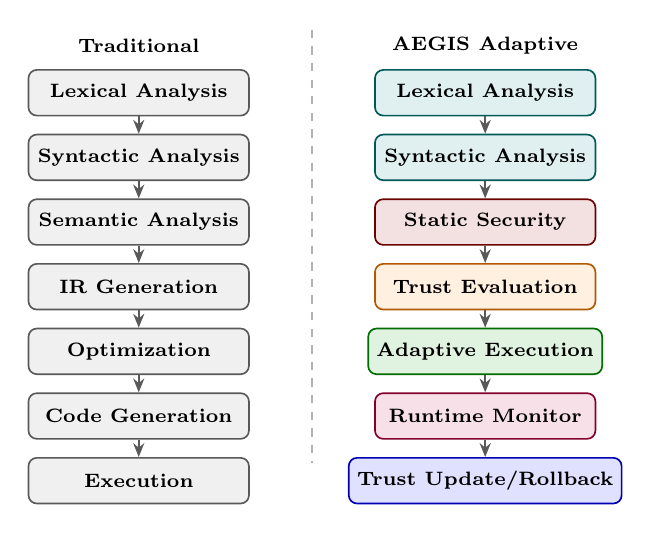
\begin{tikzpicture}[node distance=0.22cm,
                    every node/.style={font=\scriptsize}]

  %% ---- Traditional Pipeline (left) ----
  \node[font=\scriptsize\bfseries] at (-2.0,0.3) {Traditional};
  \node[stage=gray,   minimum width=2.8cm] (t1) at (-2.0,-0.3)
       {Lexical Analysis};
  \node[stage=gray,   minimum width=2.8cm, below=of t1] (t2)
       {Syntactic Analysis};
  \node[stage=gray,   minimum width=2.8cm, below=of t2] (t3)
       {Semantic Analysis};
  \node[stage=gray,   minimum width=2.8cm, below=of t3] (t4)
       {IR Generation};
  \node[stage=gray,   minimum width=2.8cm, below=of t4] (t5)
       {Optimization};
  \node[stage=gray,   minimum width=2.8cm, below=of t5] (t6)
       {Code Generation};
  \node[stage=gray,   minimum width=2.8cm, below=of t6] (t7)
       {Execution};

  \foreach \a/\b in {t1/t2, t2/t3, t3/t4, t4/t5, t5/t6, t6/t7}
    \draw[arr] (\a) -- (\b);

  %% ---- AEGIS Pipeline (right) ----
  \node[font=\scriptsize\bfseries] at (2.4,0.3) {AEGIS Adaptive};
  \node[stage=teal,   minimum width=2.8cm] (a1) at (2.4,-0.3)
       {Lexical Analysis};
  \node[stage=teal,   minimum width=2.8cm, below=of a1] (a2)
       {Syntactic Analysis};
  \node[stage=red!60!black, minimum width=2.8cm, below=of a2] (a3)
       {Static Security};
  \node[stage=orange, minimum width=2.8cm, below=of a3] (a4)
       {Trust Evaluation};
  \node[stage=green!60!black, minimum width=2.8cm, below=of a4] (a5)
       {Adaptive Execution};
  \node[stage=purple, minimum width=2.8cm, below=of a5] (a6)
       {Runtime Monitor};
  \node[stage=blue,   minimum width=2.8cm, below=of a6] (a7)
       {Trust Update/Rollback};

  \foreach \a/\b in {a1/a2, a2/a3, a3/a4, a4/a5, a5/a6, a6/a7}
    \draw[arr] (\a) -- (\b);

  %% Divider
  \draw[dashed, black!30, line width=0.6pt] (0.2,0.5) -- (0.2,-5.0);

\end{tikzpicture}
\caption{Pipeline Comparison.}
\label{fig:pipeline_compare}
\end{figure}
%% ---- END FIGURE 5 --------------------------------------------------

\subsection{Security Mechanisms in Code Execution}

\textbf{Sandboxing.}  The basic idea is straightforward: confine
the running program so it cannot touch files, networks, or memory
regions outside a designated area.  Hardware-backed sandboxes
like Intel SGX enclaves~\cite{menetrey2024sgx} and WebAssembly
runtimes~\cite{johnson2023wave,lehmann2020wasm,wasm_survey2024,tang2023wasm_runtimes}
push this enforcement down to the instruction level, which
produces strong guarantees at the price of per-instruction
bounds checking and a restricted system-call surface.

\textbf{Static code analysis.}  Rather than confining a
running program, static tools inspect the source or an
intermediate representation \emph{before} any instruction
executes.  They can catch buffer overflows, undefined-variable
accesses, and literal divisions by
zero~\cite{jiang2020elaid,khoury2022buffer}.  The catch is
that undecidability forces every analyzer to choose between
false positives (flagging correct code) and false negatives
(missing real bugs); practitioners consistently find the
latter more
dangerous~\cite{ami2024false_neg,huang2024static}.

\textbf{Runtime monitoring.}  Dynamic techniques---instruction
counting, memory-bounds checking, taint tracking, assertion
verification~\cite{wang2022vulnets}---observe actual behavior
while the program runs.  They pick up exactly the violations
that static analysis cannot see: data-dependent infinite loops,
overflow conditions triggered only by particular input values,
and resource exhaustion that depends on workload size.  The
trade-off is per-instruction overhead, which can become
significant for tight inner loops.

\subsection{Trust Models and Adaptive Runtime Systems}

\textbf{Trust-based models} assign a numerical score to an
entity---user, device, or, in our case, program---and adjust
that score up or down based on observed behavior.  The score
then gates access to resources or
privileges~\cite{wang2022trust,li2022iot_trust,fernandez2024sla}.
IoT and distributed-systems research has applied this idea to
authentication, service selection, and reputation
management~\cite{ullah2024deeptrust}.  AEGIS borrows the
mechanism but applies it within a single-node interpreter,
where the ``privilege'' being managed is the right to run on
a faster execution path.

\textbf{Adaptive runtimes} change their behavior based on what
they observe.  The best-known example is JIT compilation,
where hot code paths graduate from interpretation to compiled
execution as profiling data
accumulates~\cite{qin2022jit_security,chen2024jit_val}.  The
key difference from AEGIS is what triggers the promotion: JIT
compilers use execution \emph{frequency}; AEGIS uses
\emph{violation absence}.
Figure~\ref{fig:concept_flow} illustrates how these background
concepts feed into the AEGIS design.

%% ---- FIGURE 6: Background Concept Relationships --------------------
\begin{figure}[t]
\centering
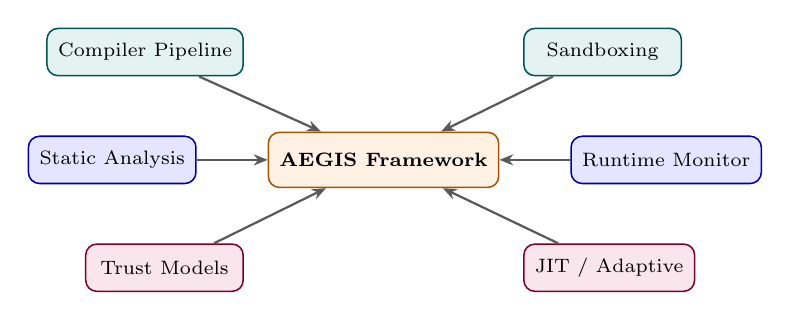
\begin{tikzpicture}[every node/.style={font=\scriptsize},
                    node distance=0.55cm and 0.6cm]

  %% Central node
  \node[rbox=orange, minimum width=2.2cm, minimum height=0.7cm,
        font=\scriptsize\bfseries] (aegis) {AEGIS Framework};

  %% Surrounding concepts
  \node[rbox=teal,   minimum width=2.0cm, above left=0.7cm and 0.3cm of aegis]
       (comp) {Compiler Pipeline};
  \node[rbox=teal,   minimum width=2.0cm, above right=0.7cm and 0.3cm of aegis]
       (sand) {Sandboxing};
  \node[rbox=blue,   minimum width=2.0cm, left=0.9cm of aegis]
       (static) {Static Analysis};
  \node[rbox=blue,   minimum width=2.0cm, right=0.9cm of aegis]
       (runtime) {Runtime Monitor};
  \node[rbox=purple, minimum width=2.0cm, below left=0.7cm and 0.3cm of aegis]
       (trust) {Trust Models};
  \node[rbox=purple, minimum width=2.0cm, below right=0.7cm and 0.3cm of aegis]
       (jit) {JIT / Adaptive};

  %% Arrows
  \draw[arr] (comp)    -- (aegis);
  \draw[arr] (sand)    -- (aegis);
  \draw[arr] (static)  -- (aegis);
  \draw[arr] (runtime) -- (aegis);
  \draw[arr] (trust)   -- (aegis);
  \draw[arr] (jit)     -- (aegis);

\end{tikzpicture}
\caption{Concept Map.}
\label{fig:concept_flow}
\end{figure}
%% ---- END FIGURE 6 --------------------------------------------------

%% ====================================================================
\section{Related Work}
\label{sec:related}
%% ====================================================================

\subsection{Sandboxing and Isolation}

WebAssembly has become the go-to technology for portable,
sandboxed execution.  Johnson et~al.\ built WaVe, a Wasm
sandboxing runtime whose isolation properties come with
machine-checkable proofs~\cite{johnson2023wave}.
M\'en\'etrey et~al.\ pushed the boundary further with TWINE,
which nests Wasm inside Intel SGX enclaves and adds remote
attestation while keeping overhead close to unprotected
baselines~\cite{menetrey2024sgx}.  Narayan et~al.\ addressed
a complementary threat vector: Swivel hardens Wasm against
Spectre-class transient-execution attacks by inserting
software fences at compilation time~\cite{narayan2022swivel}.
Strong as these systems are, they provide \emph{static}
isolation.  A program that runs safely a thousand times still
pays the same sandboxing cost on run one thousand and one.
AEGIS keeps the sandbox as a mandatory starting point but
relaxes it selectively once a program has accumulated enough
evidence of safe behavior.

\subsection{Static and Dynamic Analysis}

Static tools can flag integer-overflow-to-buffer-overflow
chains, undefined-variable accesses, and literal divisions by
zero before any instruction executes~\cite{jiang2020elaid}.
Yet the empirical reality, documented in a 2024 IEEE~S\&P
Distinguished Paper by Ami et~al., is that false negatives in
production-grade analyzers remain stubbornly
common~\cite{ami2024false_neg}.  Cui et~al.\ corroborate this
finding by mining the historical issue trackers of PMD,
SpotBugs, and SonarQube, revealing that root causes range from
flawed rule specifications to unhandled language
features~\cite{huang2024static}.  On the dynamic side,
Tan et~al.\ recently demonstrated MCP-SandboxScan, which
combines Wasm sandboxing with runtime taint tracking to
secure tool-augmented LLM
agents~\cite{tan2025sandboxscan}.

AEGIS occupies a middle ground: its static analyzer runs
\emph{before} execution to catch deterministic patterns,
while a runtime monitor picks up everything the static layer
cannot see (data-dependent loops, computed overflows).
The two layers together achieve complete coverage within
the defined threat surface.

\subsection{Trust and Reputation Systems}

Trust management has a long history in distributed systems.
Wang et~al.\ survey trust models across heterogeneous networks
and identify evidence accumulation and penalty severity as
the two primary design knobs~\cite{wang2022trust}.  In IoT
settings, Li et~al.\ use SLA-driven trust to select
negotiation candidates~\cite{li2022iot_trust};
Fernandez-Fernandez et~al.\ build a framework that predicts
SLA breaches in 5G service
marketplaces~\cite{fernandez2024sla}; and Ullah et~al.\
propose Deep Trust, a neural approach for continuous score
updates in IoT networks~\cite{ullah2024deeptrust}.

All of these systems operate at the \emph{network or device}
level.  To our knowledge, AEGIS is the first to relocate
dynamic trust management into a single-node program
interpreter, where the ``resource'' gated by the trust score
is execution-path selection rather than network access.

\subsection{Adaptive and JIT Compilation}

Modern JIT compilers in JVM HotSpot, V8, and PyPy achieve
impressive speedups by profiling execution frequency and
promoting hot paths to native
code~\cite{qin2022jit_security}.  Qin et~al.\ show that
this promotion mechanism can itself leak information
through timing side-channels when the decision is
data-dependent.  Li et~al.\ validate JIT correctness by
exhaustively exploring the compilation space,
uncovering 85 bugs in production
runtimes~\cite{chen2024jit_val}.

AEGIS borrows the \emph{tiered promotion} idea but
replaces the signal: where JIT compilers ask ``is this code
hot?'', AEGIS asks ``is this code safe?''  The result is
that promotion incentives align with security rather than
sitting in tension with it.

\subsection{Compiler and Interpreter Foundations}

The AEGIS pipeline follows textbook compiler
construction~\cite{aho2007compilers}: recursive-descent
parsing, visitor-pattern AST traversal, three-address-code
generation, and stack-based bytecode execution.  Wang's
characterization of standalone Wasm runtimes, which reports
1.59--9.57$\times$ slowdowns relative to native execution,
motivates the search for lighter-weight adaptive
strategies~\cite{tang2023wasm_runtimes}.  Khoury's taxonomy
of buffer-overflow-inducing software flaws informed our
static threat classification~\cite{khoury2022buffer}, and
Wang et~al.'s vulnerability-net approach to dynamic
detection complements our runtime
monitor~\cite{wang2022vulnets}.

\subsection{Summary of Gaps}

%% ---- FIGURE: Gap Summary Radar Diagram ----
\begin{figure}[t]
\centering
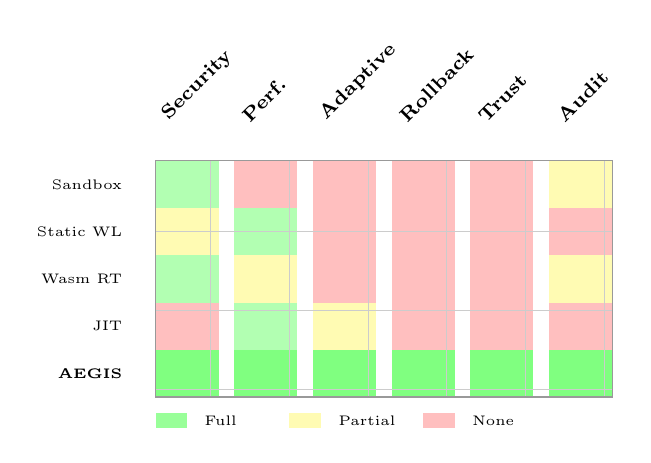
\begin{tikzpicture}[every node/.style={font=\scriptsize}]
  %% Column headers
  \node[font=\scriptsize\bfseries, rotate=45, anchor=south west]
       at (0.5,3.2) {Security};
  \node[font=\scriptsize\bfseries, rotate=45, anchor=south west]
       at (1.5,3.2) {Perf.};
  \node[font=\scriptsize\bfseries, rotate=45, anchor=south west]
       at (2.5,3.2) {Adaptive};
  \node[font=\scriptsize\bfseries, rotate=45, anchor=south west]
       at (3.5,3.2) {Rollback};
  \node[font=\scriptsize\bfseries, rotate=45, anchor=south west]
       at (4.5,3.2) {Trust};
  \node[font=\scriptsize\bfseries, rotate=45, anchor=south west]
       at (5.5,3.2) {Audit};

  %% Row labels
  \node[anchor=east, font=\tiny] at (0.0,2.6) {Sandbox};
  \node[anchor=east, font=\tiny] at (0.0,2.0) {Static WL};
  \node[anchor=east, font=\tiny] at (0.0,1.4) {Wasm RT};
  \node[anchor=east, font=\tiny] at (0.0,0.8) {JIT};
  \node[anchor=east, font=\tiny] at (0.0,0.2) {\textbf{AEGIS}};

  %% Grid fill: green=yes, red=no, yellow=partial
  %% Row 1: Sandbox
  \fill[green!30] (0.3,2.3) rectangle (1.1,2.9);  % Security
  \fill[red!25]   (1.3,2.3) rectangle (2.1,2.9);  % Perf
  \fill[red!25]   (2.3,2.3) rectangle (3.1,2.9);  % Adaptive
  \fill[red!25]   (3.3,2.3) rectangle (4.1,2.9);  % Rollback
  \fill[red!25]   (4.3,2.3) rectangle (5.1,2.9);  % Trust
  \fill[yellow!30](5.3,2.3) rectangle (6.1,2.9);  % Audit

  %% Row 2: Static WL
  \fill[yellow!30](0.3,1.7) rectangle (1.1,2.3);
  \fill[green!30] (1.3,1.7) rectangle (2.1,2.3);
  \fill[red!25]   (2.3,1.7) rectangle (3.1,2.3);
  \fill[red!25]   (3.3,1.7) rectangle (4.1,2.3);
  \fill[red!25]   (4.3,1.7) rectangle (5.1,2.3);
  \fill[red!25]   (5.3,1.7) rectangle (6.1,2.3);

  %% Row 3: Wasm RT
  \fill[green!30] (0.3,1.1) rectangle (1.1,1.7);
  \fill[yellow!30](1.3,1.1) rectangle (2.1,1.7);
  \fill[red!25]   (2.3,1.1) rectangle (3.1,1.7);
  \fill[red!25]   (3.3,1.1) rectangle (4.1,1.7);
  \fill[red!25]   (4.3,1.1) rectangle (5.1,1.7);
  \fill[yellow!30](5.3,1.1) rectangle (6.1,1.7);

  %% Row 4: JIT
  \fill[red!25]   (0.3,0.5) rectangle (1.1,1.1);
  \fill[green!30] (1.3,0.5) rectangle (2.1,1.1);
  \fill[yellow!30](2.3,0.5) rectangle (3.1,1.1);
  \fill[red!25]   (3.3,0.5) rectangle (4.1,1.1);
  \fill[red!25]   (4.3,0.5) rectangle (5.1,1.1);
  \fill[red!25]   (5.3,0.5) rectangle (6.1,1.1);

  %% Row 5: AEGIS
  \fill[green!50] (0.3,-0.1) rectangle (1.1,0.5);
  \fill[green!50] (1.3,-0.1) rectangle (2.1,0.5);
  \fill[green!50] (2.3,-0.1) rectangle (3.1,0.5);
  \fill[green!50] (3.3,-0.1) rectangle (4.1,0.5);
  \fill[green!50] (4.3,-0.1) rectangle (5.1,0.5);
  \fill[green!50] (5.3,-0.1) rectangle (6.1,0.5);

  %% Grid lines
  \draw[black!20] (0.3,-0.1) grid[step=1.0] (6.1,2.9);
  \draw[black!40] (0.3,-0.1) rectangle (6.1,2.9);

  %% Legend
  \fill[green!40] (0.3,-0.5) rectangle (0.7,-0.3);
  \node[anchor=west, font=\tiny] at (0.8,-0.4) {Full};
  \fill[yellow!30] (2.0,-0.5) rectangle (2.4,-0.3);
  \node[anchor=west, font=\tiny] at (2.5,-0.4) {Partial};
  \fill[red!25] (3.7,-0.5) rectangle (4.1,-0.3);
  \node[anchor=west, font=\tiny] at (4.2,-0.4) {None};

\end{tikzpicture}
\caption{Capability Coverage.}
\label{fig:capability_coverage}
\end{figure}

The literature addresses isolation, static detection, dynamic
trust, and adaptive execution as largely separate concerns.
Figure~\ref{fig:capability_coverage} visualizes how each
approach covers the six core capability dimensions.  No prior
system combines all four capabilities at the interpreter level
with persistent, cross-session trust and auditable per-stage
telemetry.  The distinctions are structural:

\begin{itemize}[nosep]
  \item \emph{Sandboxes}~\cite{johnson2023wave,menetrey2024sgx}
    provide static isolation with no performance adaptation.
  \item \emph{JIT compilers}~\cite{qin2022jit_security} optimize
    based on frequency, which is orthogonal to security.
  \item \emph{Static analyzers}~\cite{ami2024false_neg,huang2024static}
    cannot address runtime-dependent violations.
  \item \emph{Trust systems}~\cite{wang2022trust,ullah2024deeptrust}
    operate at the network or device level, not per-program.
\end{itemize}

\noindent AEGIS fills the intersection of these gaps.  The
following sections detail its design.

%% ====================================================================
\section{Comparative Analysis of Execution Strategies}
\label{sec:comparative}
%% ====================================================================

To place AEGIS among existing untrusted-code execution
strategies, Table~\ref{tab:expanded_compare} compares six
approaches across eight capability dimensions. The
systems listed represent the major categories from the
related work survey: traditional sandboxing, static whitelisting,
WebAssembly runtimes, JIT compilation, implicit trust execution,
and AEGIS.

\begin{table*}[t]
\caption{Comparison Matrix.}
\label{tab:expanded_compare}
\centering
\renewcommand{\arraystretch}{1.20}
\small
\begin{tabular}{@{} l c c c c c c c c @{}}
\toprule
\textbf{System / Approach} &
\textbf{Security} &
\textbf{Perf.} &
\textbf{Adaptivity} &
\textbf{Rollback} &
\textbf{Rt.\ Mon.} &
\textbf{Trust} &
\textbf{Audit} &
\textbf{Deploy.} \\
\midrule
Traditional Sandboxing
  & High & Low & None & No & Partial & No & Partial & Low \\
Static Whitelisting
  & Medium & High & None & No & No & No & No & Low \\
WebAssembly Runtime
  & High & Medium & None & No & Partial & No & Partial & Medium \\
JIT Compilation
  & Low & High & Frequency & No & No & No & No & High \\
Implicit Trust Execution
  & None & High & None & No & No & No & No & Low \\
\textbf{AEGIS (Proposed)}
  & \textbf{High} & \textbf{High}${}^{\dag}$
  & \textbf{Evidence} & \textbf{Yes}
  & \textbf{Full} & \textbf{Yes} & \textbf{Full}
  & \textbf{Low} \\
\bottomrule
\multicolumn{9}{@{}p{0.95\textwidth}@{}}{\footnotesize
${}^{\dag}$ High performance applies only to trust-promoted
programs; untrusted programs execute at sandboxed speed with
full security enforcement.}
\end{tabular}
\end{table*}

Table~\ref{tab:expanded_compare} distills the comparison into
eight capability dimensions.  The landscape it reveals is
striking: every existing strategy leaves at least three columns
blank.  Sandboxes and Wasm runtimes nail security but give up
performance and adaptivity.  JIT compilers reclaim speed through
tiered promotion, yet their signal is execution \emph{frequency}
---a quantity that says nothing about whether the code is
actually safe.  Static whitelisting avoids runtime cost but
cannot cope with previously unseen code and offers no way to
undo a wrong decision.  Implicit trust is the fastest option
and also the most reckless.

AEGIS is the only row in the table where every cell is marked
\textbf{High}, \textbf{Yes}, or \textbf{Full}.  That breadth
follows directly from the architectural choice to embed a trust
accumulation layer inside a compiler-style pipeline: the early
stages provide security, the trust gate provides adaptivity,
the dual execution path provides performance, and the rollback
handler provides recoverability.  The next sections spell out
how each piece works.

%% ====================================================================
\section{System Architecture}
\label{sec:arch}
%% ====================================================================

\subsection{Subsystem Decomposition}

AEGIS is split into three subsystems, connected by a JSON-based
REST\,API (Figure~\ref{fig:arch}).  The \textbf{Core Interpreter}
(Python~3, roughly 5\,500 lines) houses the language semantics,
the seven-stage pipeline, the trust model, and every security
check.  The \textbf{Backend Server} (Flask, about 710 lines)
wraps the core behind HTTP endpoints, handling serialization,
error normalization, and session management.  The
\textbf{Frontend IDE} (React~19, approximately 1\,330 lines)
provides a Monaco-based editor, a real-time pipeline
visualization panel, an AST tree explorer, a token stream view,
and a Recharts-based trust dashboard.

Trust persists in a single \textit{.aegis\_trust.json} file,
keyed by the first sixteen hex characters of each program's
SHA-256 hash.  The store is read at Stage~4 and written back
at Stage~6 of every run, so it survives server restarts and
carries trust across sessions.

%% ---- FIGURE 1: System Architecture ---------------------------------
\begin{figure}[t]
\centering
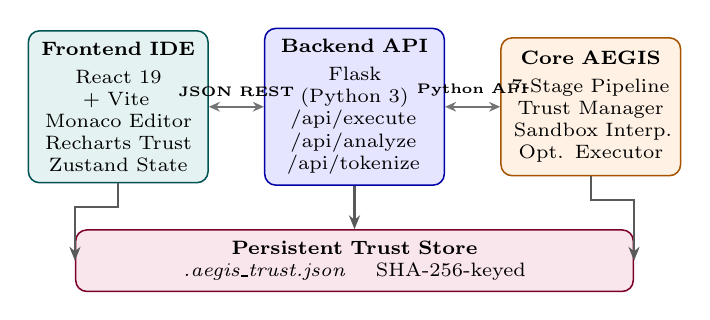
\begin{tikzpicture}[node distance=0.5cm and 0.55cm,
                    every node/.style={font=\scriptsize}]

  %% Frontend subsystem
  \node[rbox=teal, minimum width=2.1cm, minimum height=1.75cm,
        text width=2.0cm, align=center] (fe)
    {\textbf{Frontend IDE}\\[2pt]
     React 19 + Vite\\
     Monaco Editor\\
     Recharts Trust\\
     Zustand State};

  %% Backend subsystem
  \node[rbox=blue, minimum width=2.1cm, minimum height=1.75cm,
        text width=2.0cm, align=center, right=0.7cm of fe] (be)
    {\textbf{Backend API}\\[2pt]
     Flask (Python 3)\\
     /api/execute\\
     /api/analyze\\
     /api/tokenize};

  %% Core interpreter
  \node[rbox=orange, minimum width=2.1cm, minimum height=1.75cm,
        text width=2.0cm, align=center, right=0.7cm of be] (core)
    {\textbf{Core AEGIS}\\[2pt]
     7-Stage Pipeline\\
     Trust Manager\\
     Sandbox Interp.\\
     Opt. Executor};

  %% REST label
  \draw[darr] (fe) -- node[above, font=\tiny\bfseries]{JSON REST} (be);
  \draw[darr] (be) -- node[above, font=\tiny\bfseries]{Python API} (core);

  %% Trust store
  \node[rbox=purple, minimum width=6.9cm, minimum height=0.52cm,
        text width=6.8cm, align=center,
        below=0.55cm of be] (trust)
    {\textbf{Persistent Trust Store} \quad
     \textit{.aegis\_trust.json} \quad SHA-256-keyed};

  %% Lines to trust store
  \draw[arr] (fe.south)   -- ++(0,-0.3) -| (trust.west);
  \draw[arr] (be.south)   -- (trust.north);
  \draw[arr] (core.south) -- ++(0,-0.3) -| (trust.east);

\end{tikzpicture}
\caption{AEGIS Architecture.}
\label{fig:arch}
\end{figure}
%% ---- END FIGURE 1 --------------------------------------------------

\subsection{Seven-Stage Execution Pipeline}

Every code submission is processed through a fixed, sequentially
ordered seven-stage pipeline implemented in
\textit{AegisExecutionPipeline}. Table~\ref{tab:pipeline} summarizes
each stage's input, primary artifact, and error type. Stage~5
diverges into two execution paths (5a and 5b) selected by the trust
gate at Stage~4, then converges at Stage~6 for trust update and
Stage~7 for conditional rollback. Figure~\ref{fig:pipeline}
illustrates the complete data-flow.

\begin{table}[t]
\caption{Execution Pipeline.}
\label{tab:pipeline}
\centering
\renewcommand{\arraystretch}{1.18}
\small
\begin{tabular}{@{}c p{1.65cm} p{2.1cm} p{1.6cm}@{}}
\toprule
\textbf{St.} & \textbf{Name} & \textbf{Output Artifact} &
\textbf{Error Type} \\
\midrule
1  & Lexical Analysis     & Token stream              & LexicalError \\
2  & Syntax Analysis      & AST (7 node types)        & SyntaxError  \\
3  & Static Analysis      & Issues list / pass        & SemanticError\\
4  & Trust Lookup         & TrustScore, ExecMode      & ---          \\
5a & Sandboxed Interp.    & Exec.\ result (INTERP)    & RuntimeError \\
5b & Optimized Exec.      & Exec.\ result (OPT)       & RuntimeError \\
5c & Runtime Monitor      & ExecutionMetrics          & ---          \\
6  & Trust Score Update   & Updated TrustScore        & ---          \\
7  & Rollback Handler     & RollbackEvent (if any)    & ---          \\
\bottomrule
\end{tabular}
\end{table}

%% ---- FIGURE 2: Pipeline Data-Flow ----------------------------------
\begin{figure}[t]
\centering
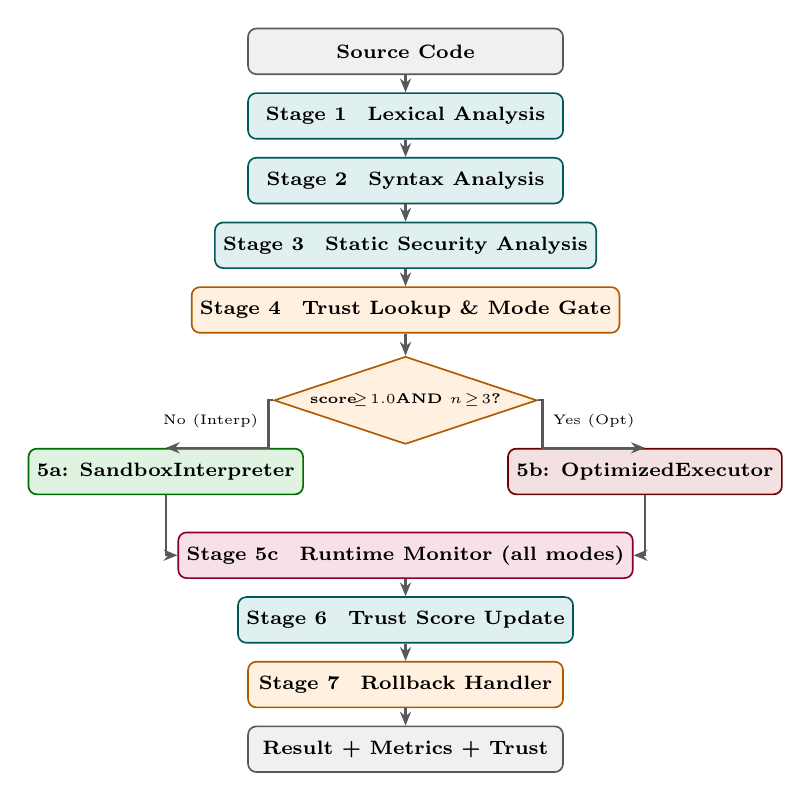
\begin{tikzpicture}[node distance=0.24cm,
                    every node/.style={font=\scriptsize}]

  %% Source
  \node[stage=gray, minimum width=4.0cm] (src)
        {\textsc{Source Code}};

  %% Stages 1-4
  \node[stage=teal,   minimum width=4.0cm, below=0.22cm of src] (s1)
        {Stage 1 \enspace Lexical Analysis};
  \node[stage=teal,   minimum width=4.0cm, below=0.22cm of s1]  (s2)
        {Stage 2 \enspace Syntax Analysis};
  \node[stage=teal,   minimum width=4.0cm, below=0.22cm of s2]  (s3)
        {Stage 3 \enspace Static Security Analysis};
  \node[stage=orange, minimum width=4.0cm, below=0.22cm of s3]  (s4)
        {Stage 4 \enspace Trust Lookup \& Mode Gate};

  %% Decision diamond
  \node[diam, below=0.28cm of s4] (dec)
        {score$\!\geq\!1.0$\\AND $n\!\geq\!3$?};

  %% Branch nodes
  \node[stage=green!60!black, minimum width=1.72cm,
        below left=0.32cm and 0.45cm of dec] (s5a)
        {5a: Sandbox\\Interpreter};
  \node[stage=red!60!black, minimum width=1.72cm,
        below right=0.32cm and 0.45cm of dec] (s5b)
        {5b: Optimized\\Executor};

  %% Runtime monitor
  \node[stage=purple, minimum width=4.0cm, below=1.1cm of dec] (s5c)
        {Stage 5c \enspace Runtime Monitor (all modes)};

  %% Stages 6-7
  \node[stage=teal,   minimum width=4.0cm, below=0.22cm of s5c] (s6)
        {Stage 6 \enspace Trust Score Update};
  \node[stage=orange, minimum width=4.0cm, below=0.22cm of s6]  (s7)
        {Stage 7 \enspace Rollback Handler};

  %% Result
  \node[stage=gray,   minimum width=4.0cm, below=0.22cm of s7]  (res)
        {\textsc{Result + Metrics + Trust}};

  %% Straight arrows
  \foreach \a/\b in {src/s1, s1/s2, s2/s3, s3/s4, s4/dec,
                     s5c/s6, s6/s7, s7/res}
    \draw[arr] (\a) -- (\b);

  %% Branch arrows
  \draw[arr] (dec.west) -- ++(-0.06,0)
             |- node[left, pos=0.22, font=\tiny]{No (Interp)} (s5a.north);
  \draw[arr] (dec.east) -- ++(0.06,0)
             |- node[right,pos=0.22, font=\tiny]{Yes (Opt)} (s5b.north);

  %% Converge into monitor
  \draw[arr] (s5a.south) |- (s5c.west);
  \draw[arr] (s5b.south) |- (s5c.east);

\end{tikzpicture}
\caption{AEGIS Pipeline.}
\label{fig:pipeline}
\end{figure}
%% ---- END FIGURE 2 --------------------------------------------------

\subsection{Detailed Execution Lifecycle}

Figure~\ref{fig:lifecycle_flow} presents the complete execution
lifecycle as a flowchart, detailing the control flow from code
submission to output generation. The lifecycle begins when the
user submits source code through the web IDE or REST API. The
frontend serializes the code as a JSON payload and dispatches it
to the \textit{/api/execute} endpoint. The backend deserializes
the request and instantiates the
\textit{AegisExecutionPipeline}, which orchestrates the
seven-stage processing.

\textbf{Stages~1--3 (Frontend Analysis).} The pipeline first
invokes the \textit{Lexer} to tokenize the input, producing a
token stream that encodes each lexeme with its type, value,
line, and column. The \textit{Parser} consumes this stream via
backtracking-free recursive descent, constructing a homogeneous
AST over seven node types. The \textit{StaticAnalyzer} then
walks the AST via the visitor pattern, accumulating all
diagnostic issues. If any HIGH-severity issue is found, the
pipeline halts and returns the diagnostic set.

\textbf{Stage~4 (Trust Gate).} The pipeline computes the
SHA-256 hash of the source code and queries the
\textit{TrustManager} for the corresponding
\textit{TrustScore}. The mode selection function
(Eq.~\ref{eq:mode}) evaluates whether the program qualifies
for optimized execution.

\textbf{Stages~5a/5b (Dual Execution).} Based on the trust
gate decision, the pipeline dispatches to either the
\textit{SandboxedInterpreter} (tree-walking with full
enforcement) or the \textit{OptimizedExecutor} (AST
optimization followed by cached execution). Both paths
operate under the \textit{RuntimeMonitor}, which instruments
every AST node visit with instruction counting, arithmetic
bounds checking, and loop iteration tracking.

\textbf{Stages~6--7 (Feedback Loop).} After execution completes,
the \textit{TrustManager} applies the increment or decrement
schedule based on execution metrics and violation status. If
violations were detected during optimized execution, the
\textit{RollbackHandler} performs cache invalidation, trust
revocation, and event recording in a single atomic operation.

%% ---- FIGURE 7: Execution Lifecycle Flowchart -----------------------
\begin{figure}[t]
\centering
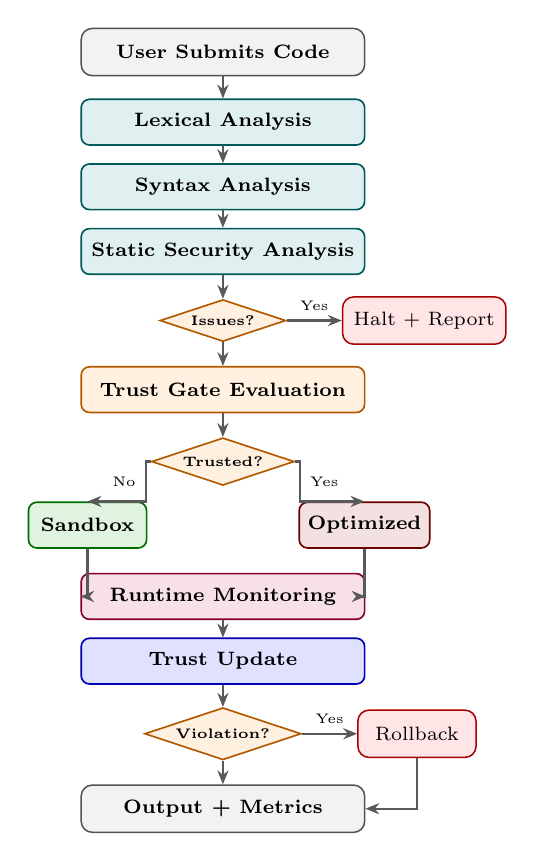
\begin{tikzpicture}[node distance=0.22cm,
                    every node/.style={font=\scriptsize}]

  \node[rbox=gray, minimum width=3.6cm] (input)
       {\textbf{User Submits Code}};

  \node[stage=teal, minimum width=3.6cm, below=0.28cm of input] (lex)
       {Lexical Analysis};
  \node[stage=teal, minimum width=3.6cm, below=of lex] (parse)
       {Syntax Analysis};
  \node[stage=teal, minimum width=3.6cm, below=of parse] (sstat)
       {Static Security Analysis};

  \node[diam, below=0.3cm of sstat] (safe) {Issues?};

  \node[rbox=red, minimum width=1.5cm, right=0.7cm of safe] (halt)
       {Halt + Report};

  \node[stage=orange, minimum width=3.6cm, below=0.3cm of safe] (tgate)
       {Trust Gate Evaluation};
  \node[diam, below=0.3cm of tgate] (trusted) {Trusted?};

  \node[stage=green!60!black, minimum width=1.5cm,
        below left=0.35cm and 0.5cm of trusted] (sand)
       {Sandbox};
  \node[stage=red!60!black, minimum width=1.5cm,
        below right=0.35cm and 0.5cm of trusted] (opt)
       {Optimized};

  \node[stage=purple, minimum width=3.6cm, below=1.1cm of trusted] (mon)
       {Runtime Monitoring};
  \node[stage=blue, minimum width=3.6cm, below=of mon] (tupd)
       {Trust Update};
  \node[diam, below=0.28cm of tupd] (viol) {Violation?};

  \node[rbox=red, minimum width=1.5cm, right=0.7cm of viol] (roll)
       {Rollback};

  \node[rbox=gray, minimum width=3.6cm, below=0.3cm of viol] (out)
       {\textbf{Output + Metrics}};

  %% Arrows
  \foreach \a/\b in {input/lex, lex/parse, parse/sstat, sstat/safe,
                     safe/tgate, tgate/trusted, mon/tupd, tupd/viol,
                     viol/out}
    \draw[arr] (\a) -- (\b);

  \draw[arr] (safe.east) -- node[above,font=\tiny]{Yes} (halt);
  \draw[arr] (trusted.west) -- ++(-0.06,0)
             |- node[left,pos=0.25,font=\tiny]{No} (sand.north);
  \draw[arr] (trusted.east) -- ++(0.06,0)
             |- node[right,pos=0.25,font=\tiny]{Yes} (opt.north);
  \draw[arr] (sand.south) |- (mon.west);
  \draw[arr] (opt.south)  |- (mon.east);
  \draw[arr] (viol.east) -- node[above,font=\tiny]{Yes} (roll);
  \draw[arr] (roll.south) |- (out.east);

\end{tikzpicture}
\caption{Execution Flow.}
\label{fig:lifecycle_flow}
\end{figure}
%% ---- END FIGURE 7 --------------------------------------------------

\subsection{Subsystem Interaction Model}

The interaction between AEGIS subsystems follows a layered
architecture pattern. The \textit{Frontend IDE} communicates
exclusively with the \textit{Backend API} through JSON REST
calls; it has no direct access to the core interpreter or trust
store. The \textit{Backend API} deserializes requests, invokes
the \textit{AegisExecutionPipeline}, and serializes responses.
Within the core, the pipeline orchestrates all component
interactions: the \textit{Lexer} feeds the \textit{Parser}, whose
AST output is consumed by both the \textit{StaticAnalyzer} and
the execution engines. The \textit{TrustManager} reads and writes
the persistent trust store and provides mode decisions to the
pipeline. The \textit{RuntimeMonitor} observes both execution
engines and reports violations to the \textit{RollbackHandler},
which in turn invokes callbacks on the \textit{TrustManager}
and \textit{CodeCache} to perform trust revocation and cache
invalidation respectively.

\subsection{Language Specification}

The AEGIS language is a minimal, statically scoped, single-type
imperative language built to keep research concerns transparent
over expressiveness. The type system contains exactly one type:
32-bit signed integer, eliminating type-confusion
vulnerabilities by construction. The grammar is expressed in EBNF
with five operator precedence levels (highest to lowest):
unary minus, multiplicative ($*,\,/,\,\%$), additive ($+,\,-$),
comparison ($\!=\!,\,!=\!,\,<,\,\leq,\,>,\,\geq$), and assignment.
The token vocabulary comprises identifiers, integer literals, eleven
operators, the four control-flow keywords (\textit{if},
\textit{else}, \textit{while}, \textit{end}), the \textit{print}
statement, and structural tokens (NEWLINE, EOF).
Hash-prefixed comments are stripped during lexical analysis and
produce no tokens.

\subsection{Lexer and Parser}

The \textit{Lexer} class performs single-pass character scanning in
$O(n)$ time with two-character lookahead for compound operators
($=\!=$, $!=$, $\leq$, $\geq$) and maintains 1-indexed
line/column tracking throughout for precise error localization.
The \textit{Parser} implements backtracking-free recursive descent
in $O(m)$ token-stream time, constructing a homogeneous AST over
seven node types: \textit{IntegerNode}, \textit{IdentifierNode},
\textit{BinaryOpNode}, \textit{UnaryOpNode},
\textit{AssignmentNode}, \textit{PrintNode}, \textit{IfNode}, and
\textit{WhileNode}. Space complexity is $O(d)$ where $d$ is maximum
AST nesting depth.

\subsection{Static Security Analysis (Stage 3)}

The \textit{StaticAnalyzer} walks the AST via the visitor pattern,
accumulating all issues before raising, to provide a complete
diagnostic set in a single pass. It checks five threat classes
(Table~\ref{tab:static}). Branch analysis is intentionally
\emph{conservative}: a variable defined only in the body of an
\textit{if}-branch without a corresponding definition in the
\textit{else}-branch is not promoted to the enclosing scope. This
prevents false-safe analysis in which a later reference to a
conditionally defined variable would pass without warning.

\begin{table}[t]
\caption{Static Threat Classes.}
\label{tab:static}
\centering
\renewcommand{\arraystretch}{1.18}
\small
\begin{tabular}{@{} p{2.15cm} c p{3.15cm} @{}}
\toprule
\textbf{Threat Class} & \textbf{Sev.} & \textbf{Detection Method} \\
\midrule
Undefined Variable    & HIGH   & CFG dataflow; conservative branch
                                 join \\[2pt]
Literal Div-by-Zero   & HIGH   & Pattern: \textit{expr\,/\,IntNode(0)}
                                 \\[2pt]
Always-True Loop      & HIGH   & Detect \textit{while} with literal
                                 non-zero condition \\[2pt]
Deep Expr.\ Nesting   & MEDIUM & Recursive depth counter; max\,=\,10
                                 \\[2pt]
Large Literal Arith.  & MEDIUM & Operand magnitude $>10^{6}$ in
                                 $*$ or $+$ \\
\bottomrule
\end{tabular}
\end{table}

\subsection{Dual Execution Engines (Stages 5a and 5b)}

\textbf{Sandboxed Interpreter (Stage~5a).} The
\textit{SandboxedInterpreter} tree-walks the AST via the visitor
pattern, enforcing: a maximum of 50,000 total operations per
execution; a maximum of 10,000 iterations per \textit{while} loop;
arithmetic result clamping to the 32-bit signed integer range
$[-2^{31},\,2^{31}-1]$; and per-execution variable namespace
isolation. No file system, network, or subprocess access is defined
in the language; the attack surface is thus bounded by the language
semantics themselves.

\textbf{Optimized Executor (Stage~5b).} When the trust gate
passes, \textit{OptimizedExecutor} invokes the
\textit{ASTOptimizer} to apply four
transformations before execution: (i)~\emph{constant folding}
evaluates all-literal sub-expressions at compile time; (ii)~\emph{dead
code elimination} removes assignments whose left-hand variables are
never read; (iii)~\emph{variable propagation} substitutes
references to constant-valued variables with their literal values,
enabling further folding; and (iv)~\emph{expression simplification}
applies algebraic identities ($x+0\to x$, $x\cdot1\to x$,
$x\cdot0\to0$). The resulting optimized AST is cached in an LRU
store (capacity 100 entries, TTL 24\,h); cache hits skip
re-optimization on subsequent runs, amortizing compilation overhead
across the trust-accumulation period.

%% ====================================================================
\section{Trust Model}
\label{sec:trust}
%% ====================================================================

\subsection{TrustScore Structure}

Every program that enters the AEGIS pipeline is identified by a
16-character prefix of its SHA-256 source hash. The system maintains
a \textit{TrustScore} record per hash containing: the current
numerical score $s \in [0.0,\,10.0]$, a total execution count $n$,
a successful-execution count $n_s$, a violation count $n_v$, and a
rolling window of the last 50 execution summaries. Records are
serialized to \textit{.aegis\_trust.json} after every execution,
providing cross-session persistence and an auditable history.

Programs begin at $s = 0.0$. Trust is never granted implicitly
based on source provenance, author identity, or static analysis
outcome alone; the zero-trust default is inviolable.

\subsection{Trust Increment Schedule}

On a successful execution (no violations detected, no runtime
exceptions), the system applies a set of additive increments
according to Table~\ref{tab:increment}. The schedule is intentionally
multi-component: a program that executes efficiently (fewer than 100
instructions) \emph{and} quickly (under 0.1\,s) accumulates trust
nearly twice as fast as a program that merely avoids violations at
the base rate. Over time, programs with a sustained clean execution
history ($> 5$ successful runs) receive an additional consistency
bonus, rewarding persistent good behavior.

\begin{table}[t]
\caption{Trust Increments.}
\label{tab:increment}
\centering
\renewcommand{\arraystretch}{1.18}
\small
\begin{tabular}{@{} p{4.3cm} c @{}}
\toprule
\textbf{Condition} & \textbf{Increment} \\
\midrule
Successful execution (base reward)               & $+0.10$ \\
History bonus: $> 5$ successful executions       & $+0.05$ \\
Efficiency bonus: $<\!100$ instructions executed & $+0.02$ \\
Latency bonus: execution time $<\!0.1\,\text{s}$& $+0.02$ \\
\midrule
\textbf{Maximum per-execution gain}              & $\mathbf{+0.19}$\\
\bottomrule
\end{tabular}
\end{table}

\subsection{Trust Decrement and Penalty}

When one or more security violations are detected:
\begin{equation}
  \Delta s_{\text{viol}} =
  \begin{cases}
    -0.50 & \text{first violation in this execution} \\
    -0.20 & \text{each additional violation}
  \end{cases}
  \label{eq:penalty}
\end{equation}
with $s$ clamped to $[0.0,\,10.0]$. A single violation imposes a
penalty of $-0.50$, requiring at minimum five subsequent fully clean
executions (each earning $+0.10$ base) to recover. This asymmetry
is deliberate: it penalizes programs that exhibit even infrequent
unsafe behavior more heavily than the na\"ive penalty-to-reward ratio
implies, because the recovery cost includes the time during which
the program operates in the slower sandboxed mode.

\subsection{Mode Selection and Promotion Threshold}

Mode selection at Stage~4 is governed by:
\begin{equation}
  \text{mode}(s, n) =
  \begin{cases}
    \textsc{Optimized}   & \text{if } s \geq 1.0 \;\wedge\; n \geq 3 \\
    \textsc{Interpreted} & \text{otherwise}
  \end{cases}
  \label{eq:mode}
\end{equation}

The dual condition in Eq.~(\ref{eq:mode}) serves two purposes. The
score threshold $s \geq 1.0$ ensures that absolute evidence
accumulation has occurred; the count threshold $n \geq 3$ ensures
that at least three independent observations contribute to that
evidence, guarding against programs that earn a high initial score
through a single anomalously clean execution of a trivially short
program.

\subsection{Trust Lifecycle}

Figure~\ref{fig:lifecycle} traces the trust evolution and mode
transitions for a representative program. Clean, efficient programs
(no static issues, $<\!100$ instructions) reach the optimization
threshold within two to three executions. A single runtime violation
anywhere in the execution history resets $s$ to~0.0 and forces
full trust reconstruction. The lifecycle formalization, adapted from
dynamic trust frameworks in distributed
systems~\cite{wang2022trust,ullah2024deeptrust}, demonstrates that
the AEGIS score satisfies \emph{evidence monotonicity}: absent
violations, the score is a non-decreasing function of execution
count.

%% ---- FIGURE 3: Trust Lifecycle -------------------------------------
\begin{figure}[t]
\centering
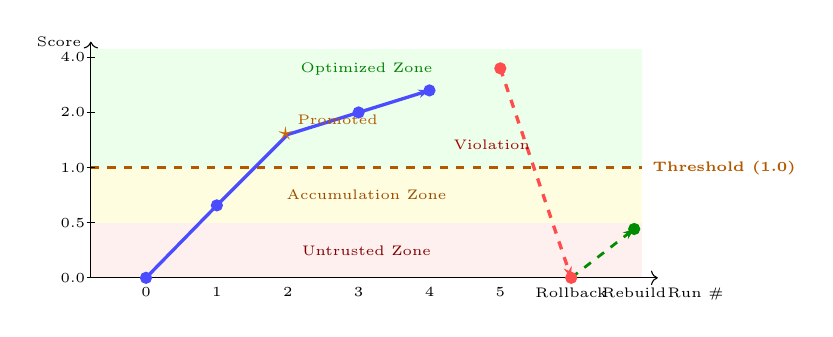
\begin{tikzpicture}[every node/.style={font=\scriptsize}]

  %% Background bands
  \fill[red!6]    (0.2, 0.0) rectangle (7.2, 0.7);
  \fill[yellow!12](0.2, 0.7) rectangle (7.2, 1.4);
  \fill[green!8]  (0.2, 1.4) rectangle (7.2, 2.9);

  %% Zone labels
  \node[font=\tiny, color=red!50!black]    at (3.7, 0.35)
       {Untrusted Zone};
  \node[font=\tiny, color=orange!60!black] at (3.7, 1.05)
       {Accumulation Zone};
  \node[font=\tiny, color=green!50!black]  at (3.7, 2.65)
       {Optimized Zone};

  %% Threshold line
  \draw[dashed, orange!70!black, line width=0.9pt]
       (0.2,1.4) -- (7.2,1.4)
       node[right, font=\tiny\bfseries, color=orange!70!black]
       {Threshold (1.0)};

  %% Y-axis
  \draw[->] (0.2,0.0) -- (0.2,3.0) node[left]{\tiny Score};
  \foreach \y/\lbl in {0.0/0.0, 0.7/0.5, 1.4/1.0, 2.1/2.0, 2.8/4.0}
    \draw (0.15,\y) -- (0.25,\y) node[left,font=\tiny]{\lbl};

  %% X-axis
  \draw[->] (0.2,0.0) -- (7.4,0.0) node[below right]{\tiny Run \#};
  \foreach \x/\lbl in {0.9/0, 1.8/1, 2.7/2, 3.6/3, 4.5/4,
                        5.4/5, 6.3/Rollback, 7.1/Rebuild}
    \node[below, font=\tiny] at (\x,0.0) {\lbl};

  %% Clean path data points: run0=0.0, 1=0.92, 2=1.82, 3=2.10, 4=2.38
  \draw[blue!70, line width=1.2pt, -{Stealth[length=4pt]}]
       (0.9,0.0) -- (1.8,0.92) -- (2.7,1.82) -- (3.6,2.10) -- (4.5,2.38);

  %% Mark promotion star at run 2 (first point >=1.4)
  \node[font=\normalsize, color=orange!80!black] at (2.7,1.82)
       {$\!\star$};
  \node[above right, font=\tiny, color=orange!70!black] at (2.7,1.82)
       {Promoted};

  %% Dots on clean path
  \foreach \x/\y in {0.9/0.0, 1.8/0.92, 3.6/2.10, 4.5/2.38}
    \filldraw[blue!70] (\x,\y) circle (2pt);

  %% Rollback: arrow plunging to 0
  \draw[red!70, line width=1.2pt, dashed, -{Stealth[length=4pt]}]
       (5.4,2.66) -- (6.3,0.0);
  \node[above left, font=\tiny, color=red!65!black] at (5.9,1.5)
       {Violation};

  %% After rollback: rebuild
  \draw[green!55!black, line width=1.0pt, dashed, -{Stealth[length=4pt]}]
       (6.3,0.0) -- (7.1,0.62);

  \filldraw[red!70]        (5.4,2.66) circle (2pt);
  \filldraw[red!70]        (6.3,0.0)  circle (2pt);
  \filldraw[green!55!black](7.1,0.62) circle (2pt);

\end{tikzpicture}
\caption{Trust Lifecycle.}
\label{fig:lifecycle}
\end{figure}
%% ---- END FIGURE 3 --------------------------------------------------

\subsection{Rollback Mechanism}

Rollback activates when: (i) the current execution mode is
OPTIMIZED, (ii) a \textit{SecurityViolation} of CRITICAL or HIGH
severity is raised by the runtime monitor, and (iii) the violation
cannot be recovered gracefully within the current execution. The
\textit{RollbackHandler} performs four atomic steps:

\begin{enumerate}
  \item \textbf{Cache invalidation:} the optimized AST entry for
        the current program hash is evicted from the LRU cache.
  \item \textbf{Trust revocation:} the TrustScore is set to~0.0
        via \textit{trust\_manager.revoke(hash)}.
  \item \textbf{Event recording:} a timestamped
        \textit{RollbackEvent} is created with fields for
        violation type, context snapshot, pre/post trust scores,
        and rollback latency; it is appended to a rolling buffer
        of the last 100 events.
  \item \textbf{Mode reversion:} the execution response marks
        mode as \textit{"optimized (rolled back)"} and forces
        subsequent executions to re-evaluate from Stage~4 under
        the reset score.
\end{enumerate}

The handler targets sub-3\,ms end-to-end latency so that rollback
does not produce a perceptible pause in interactive usage.
Figure~\ref{fig:rollback_flow} visualizes the four-step atomic
rollback procedure.

%% ---- FIGURE: Rollback Flow ------------------------------------------
\begin{figure}[t]
\centering
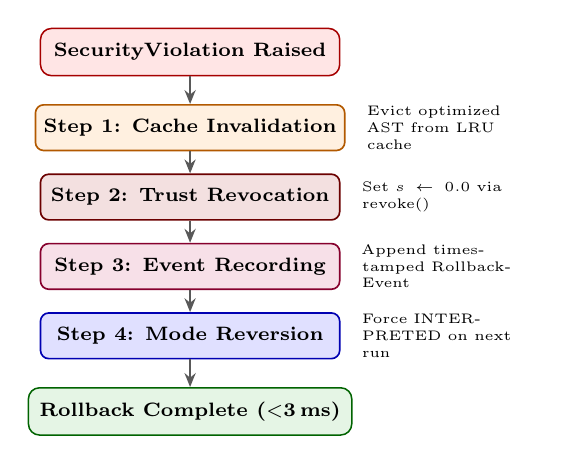
\begin{tikzpicture}[node distance=0.28cm,
                    every node/.style={font=\scriptsize}]

  \node[rbox=red, minimum width=3.8cm] (trigger)
       {\textbf{SecurityViolation Raised}};

  \node[stage=orange, minimum width=3.8cm, below=0.35cm of trigger] (s1)
       {Step 1: Cache Invalidation};
  \node[font=\tiny, right=0.15cm of s1, text width=2.2cm, align=left]
       {Evict optimized AST from LRU cache};

  \node[stage=red!60!black, minimum width=3.8cm, below=0.28cm of s1] (s2)
       {Step 2: Trust Revocation};
  \node[font=\tiny, right=0.15cm of s2, text width=2.2cm, align=left]
       {Set $s \leftarrow 0.0$ via revoke()};

  \node[stage=purple, minimum width=3.8cm, below=0.28cm of s2] (s3)
       {Step 3: Event Recording};
  \node[font=\tiny, right=0.15cm of s3, text width=2.2cm, align=left]
       {Append timestamped RollbackEvent};

  \node[stage=blue, minimum width=3.8cm, below=0.28cm of s3] (s4)
       {Step 4: Mode Reversion};
  \node[font=\tiny, right=0.15cm of s4, text width=2.2cm, align=left]
       {Force INTERPRETED on next run};

  \node[rbox=green!60!black, minimum width=3.8cm, below=0.35cm of s4] (done)
       {\textbf{Rollback Complete ($<$3\,ms)}};

  \foreach \a/\b in {trigger/s1, s1/s2, s2/s3, s3/s4, s4/done}
    \draw[arr] (\a) -- (\b);

\end{tikzpicture}
\caption{Rollback Flow.}
\label{fig:rollback_flow}
\end{figure}
%% ---- END FIGURE Rollback Flow ---------------------------------------

%% ====================================================================
\section{Security Model}
\label{sec:security}
%% ====================================================================

\subsection{Threat Model}

AEGIS targets execution environments in which code originates from
untrusted or semi-trusted parties while the execution platform
itself is assumed trusted. The threat model is intentionally
scoped to \emph{program-level} misbehavior rather than
hardware-level attacks (microarchitectural side-channels, physical
fault injection) or OS-level exploitation, which are addressed by
orthogonal mechanisms such as TEE isolation~\cite{menetrey2024sgx}.
The five threat classes considered are:

\begin{itemize}
  \setlength\itemsep{1pt}
  \item \textbf{T1 — Infinite Loops:} programs that consume CPU
        indefinitely, constituting a denial-of-service against
        the execution platform.
  \item \textbf{T2 — Integer Overflow:} arithmetic operations that
        exceed the 32-bit signed range, potentially corrupting
        control flow or producing exploitable state.
  \item \textbf{T3 — Undefined Variable Access:} reading
        uninitialized variables, which in typed languages can
        leak sensitive runtime state.
  \item \textbf{T4 — Division by Zero:} illegal arithmetic that
        terminates execution abnormally.
  \item \textbf{T5 — Resource Exhaustion:} excessive allocation of
        CPU or memory resources, degrading service for concurrent
        users.
\end{itemize}

Table~\ref{tab:threats} maps each threat class to its detection
layer and enforcement action.

\begin{table}[t]
\caption{Threat Model.}
\label{tab:threats}
\centering
\renewcommand{\arraystretch}{1.18}
\small
\begin{tabular}{@{} p{1.55cm} p{2.0cm} p{2.55cm} @{}}
\toprule
\textbf{Threat} & \textbf{Detection} & \textbf{Enforcement} \\
\midrule
Infinite loop (T1)     & Static (literal) $+$ Runtime & 10,000-iter.
                         per-loop cap \\[2pt]
Integer overflow (T2)  & Runtime bounds check  & Clamp to $[-2^{31},
                         2^{31}-1]$; abort \\[2pt]
Undefined var.\ (T3)   & Static dataflow $+$ Runtime & Immediate
                         NameError \\[2pt]
Div-by-zero (T4)       & Static (literal~0) $+$ Runtime & Execution
                         halt \\[2pt]
Resource exh.\ (T5)    & Runtime instruction counter & 50,000-op
                         global cap \\
\bottomrule
\end{tabular}
\end{table}

\subsection{Defense-in-Depth Architecture}

AEGIS organizes its security enforcement into five concentric layers.
No single layer is expected to be complete in isolation; the
combination provides coverage that no individual technique
offers~\cite{khoury2022buffer}. Figure~\ref{fig:defense} illustrates
the layered structure.

%% ---- FIGURE 4: Defense-in-Depth ------------------------------------
\begin{figure}[t]
\centering
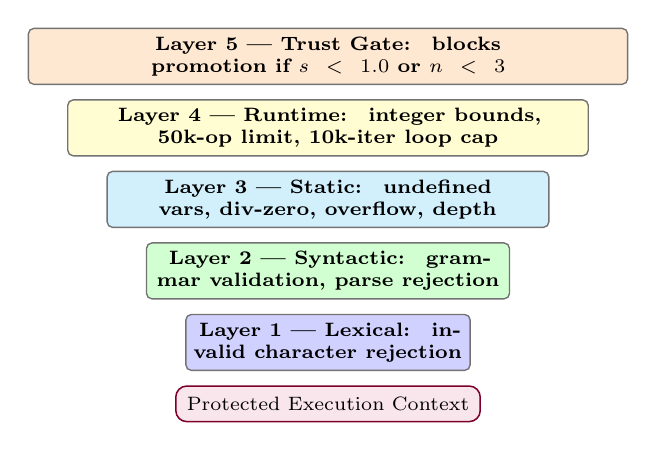
\begin{tikzpicture}[every node/.style={font=\scriptsize},
                    node distance=0.2cm]

  \node[dlayer=orange, minimum width=7.6cm, text width=7.4cm]
       (l5) at (0,0)
       {Layer 5 — Trust Gate: \ blocks promotion if $s\!<\!1.0$
        or $n\!<\!3$};

  \node[dlayer=yellow, minimum width=6.6cm, text width=6.4cm,
        below=0.18cm of l5] (l4)
       {Layer 4 — Runtime: \ integer bounds, 50k-op limit,
        10k-iter loop cap};

  \node[dlayer=cyan, minimum width=5.6cm, text width=5.4cm,
        below=0.18cm of l4] (l3)
       {Layer 3 — Static: \ undefined vars, div-zero, overflow,
        depth};

  \node[dlayer=green, minimum width=4.6cm, text width=4.4cm,
        below=0.18cm of l3] (l2)
       {Layer 2 — Syntactic: \ grammar validation, parse
        rejection};

  \node[dlayer=blue, minimum width=3.6cm, text width=3.4cm,
        below=0.18cm of l2] (l1)
       {Layer 1 — Lexical: \ invalid character rejection};

  \node[rbox=purple, minimum width=2.4cm, minimum height=0.44cm,
        below=0.18cm of l1] (core)
       {Protected Execution Context};

\end{tikzpicture}
\caption{Defense Layers.}
\label{fig:defense}
\end{figure}
%% ---- END FIGURE 4 --------------------------------------------------

\subsection{Formal Security Guarantees}

Under the AEGIS threat model and language semantics, we state five
formal guarantees:

\begin{enumerate}
  \item[\textbf{G1.}] \textbf{Namespace Isolation.} Each execution
    context $\mathcal{C}$ maintains a distinct variable store
    $\sigma_\mathcal{C}$; no variable binding is shared or leaked
    between executions.

  \item[\textbf{G2.}] \textbf{Arithmetic Safety.} Every arithmetic
    operation $\oplus$ checks its result $r$ against
    $[-2^{31},\,2^{31}-1]$; if $r$ falls outside this range, a
    \textit{SecurityViolation} is raised before any result is stored.
    Silent integer wraparound is structurally impossible.

  \item[\textbf{G3.}] \textbf{Termination.} Every execution
    terminates within 50,000 operations. The instruction counter is
    incremented on every AST node visit; when it reaches 50,000 the
    interpreter raises \textit{InstructionLimitExceeded}, halting
    execution unconditionally.

  \item[\textbf{G4.}] \textbf{Trust Monotonicity.} For a program
    $P$ whose every execution is violation-free,
    $s_t \leq s_{t+1}$ for all $t$, i.e., the trust score is
    non-decreasing over time.

  \item[\textbf{G5.}] \textbf{Rollback Completeness.} For any
    execution of $P$ in OPTIMIZED mode that raises a
    \textit{SecurityViolation}, the rollback handler resets
    $s \leftarrow 0.0$, evicts the cache entry, and marks all
    subsequent executions to restart in INTERPRETED mode.
\end{enumerate}

%% ====================================================================
\section{Algorithm Design}
\label{sec:algorithms}
%% ====================================================================

This section formalizes the core algorithms that drive the AEGIS
execution model. Three algorithms are presented: the main
adaptive execution algorithm, the trust score update procedure,
and the rollback handling mechanism.

\subsection{Adaptive Execution Algorithm}

Algorithm~\ref{alg:adaptive} describes the main execution logic.
The algorithm accepts source code and returns an execution result
comprising output, metrics, and updated trust information.

\begin{algorithm}[t]
\caption{Adaptive Execution.}
\label{alg:adaptive}
\begin{algorithmic}[1]
\Require Source code $C$, Trust threshold $\tau$, Count threshold $k$
\Ensure Execution result $R$
\State $T \gets \textsc{Tokenize}(C)$
\If{$T$ contains lexical errors}
  \State \Return $\textsc{Error}(\text{LexicalError})$
\EndIf
\State $\mathit{AST} \gets \textsc{Parse}(T)$
\State $\mathit{issues} \gets \textsc{StaticAnalyze}(\mathit{AST})$
\If{$\mathit{issues}$ contains HIGH severity}
  \State \Return $\textsc{Error}(\text{SemanticError}, \mathit{issues})$
\EndIf
\State $h \gets \textsc{SHA256}(C)[0{:}16]$
\State $(s, n) \gets \textsc{TrustLookup}(h)$
\If{$s \geq \tau$ \textbf{and} $n \geq k$}
  \State $R \gets \textsc{OptimizedExec}(\mathit{AST}, h)$
\Else
  \State $R \gets \textsc{SandboxExec}(\mathit{AST})$
\EndIf
\State $R.\mathit{metrics} \gets \textsc{Monitor}(R)$
\State $\textsc{UpdateTrust}(h, R.\mathit{metrics})$
\If{$R$ contains violations \textbf{and} mode = OPT}
  \State $\textsc{Rollback}(h)$
\EndIf
\State \Return $R$
\end{algorithmic}
\end{algorithm}

\textbf{Complexity.} The time complexity of Algorithm~\ref{alg:adaptive}
is $O(n + m + d + e)$ where $n$ is source length (lexing), $m$ is
token count (parsing), $d$ is AST depth (static analysis), and $e$
is the number of executed instructions. The space complexity is
$O(m + d + v)$ where $v$ is the number of variables in scope.

\subsection{Trust Score Update Algorithm}

Algorithm~\ref{alg:trust} formalizes the trust increment and
decrement schedule. The multi-component increment structure
ensures that programs demonstrating both static cleanliness and
runtime efficiency accumulate trust faster than programs that
merely avoid violations.

\begin{algorithm}[t]
\caption{Trust Update.}
\label{alg:trust}
\begin{algorithmic}[1]
\Require Hash $h$, Metrics $M$, Violations $V$
\Ensure Updated score $s'$
\State $(s, n, n_s, n_v) \gets \textsc{TrustLookup}(h)$
\If{$|V| > 0$} \Comment{Violations detected}
  \State $\Delta \gets -0.50 - 0.20 \cdot (|V| - 1)$
  \State $n_v \gets n_v + |V|$
\Else \Comment{Clean execution}
  \State $\Delta \gets 0.10$ \Comment{Base reward}
  \If{$n_s > 5$ successful executions}
    \State $\Delta \gets \Delta + 0.05$
  \EndIf
  \If{$M.\mathit{instructions} < 100$}
    \State $\Delta \gets \Delta + 0.02$
  \EndIf
  \If{$M.\mathit{time} < 0.1\,\text{s}$}
    \State $\Delta \gets \Delta + 0.02$
  \EndIf
  \State $n_s \gets n_s + 1$
\EndIf
\State $s' \gets \textsc{Clamp}(s + \Delta,\; 0.0,\; 10.0)$
\State $n \gets n + 1$
\State $\textsc{Persist}(h, s', n, n_s, n_v)$
\State \Return $s'$
\end{algorithmic}
\end{algorithm}

\subsection{Rollback Handling Algorithm}

Algorithm~\ref{alg:rollback} details the atomic rollback
procedure. The four steps---cache invalidation, trust
revocation, event recording, and mode reversion---execute
as a single logical transaction to prevent inconsistent state.

\begin{algorithm}[t]
\caption{Rollback Handler.}
\label{alg:rollback}
\begin{algorithmic}[1]
\Require Hash $h$, Violation $v$, Pre-score $s_{\text{pre}}$
\Ensure RollbackEvent $E$
\State $t_{\text{start}} \gets \textsc{Now}()$
\State $\textsc{CacheEvict}(h)$ \Comment{Step 1: Invalidate}
\State $\textsc{TrustRevoke}(h) \Rightarrow s \gets 0.0$ \Comment{Step 2}
\State $E \gets \textsc{CreateEvent}(v, h, s_{\text{pre}}, 0.0)$
\State $\textsc{AppendToHistory}(E)$ \Comment{Step 3: Record}
\State $\textsc{SetMode}(h, \text{INTERPRETED})$ \Comment{Step 4}
\State $E.\mathit{latency} \gets \textsc{Now}() - t_{\text{start}}$
\State \Return $E$
\end{algorithmic}
\end{algorithm}

The rollback procedure targets sub-3\,ms latency. Since all
operations are in-memory (cache eviction is a dictionary deletion,
trust revocation is a field assignment, and event recording is
a list append), the procedure avoids I/O on the critical path.
The trust store is persisted asynchronously after the rollback
completes.

The overall runtime overhead of the trust management subsystem
is bounded by $O(1)$ per execution for trust lookup and update,
as both operations involve a single dictionary access keyed by
the 16-character program hash. The space overhead is $O(p)$
where $p$ is the number of distinct programs in the trust store.

%% ====================================================================
\section{Input/Output Representation}
\label{sec:io}
%% ====================================================================

This section illustrates the transformation artifacts produced
at each stage of the AEGIS pipeline through a concrete example.

\subsection{Example Input Program}

Consider the following AEGIS program that computes the sum of
integers from 1 to 10:

\begin{lstlisting}[caption={Example AEGIS input program},
                   label={lst:input}]
# Sum of 1 to 10
total = 0
i = 1
while i <= 10
  total = total + i
  i = i + 1
end
print total
\end{lstlisting}

\subsection{Token Stream Output (Stage 1)}

Table~\ref{tab:tokens} shows a representative subset of the
token stream produced by lexical analysis of the program in
Listing~\ref{lst:input}.

\begin{table}[t]
\caption{Token Stream.}
\label{tab:tokens}
\centering
\renewcommand{\arraystretch}{1.15}
\small
\begin{tabular}{@{} c l l c c @{}}
\toprule
\textbf{\#} & \textbf{Type} & \textbf{Value} &
\textbf{Line} & \textbf{Col} \\
\midrule
1  & IDENTIFIER & \textit{total}  & 2 & 1 \\
2  & ASSIGN     & \textit{=}      & 2 & 7 \\
3  & INTEGER    & \textit{0}      & 2 & 9 \\
4  & NEWLINE    & ---             & 2 & 10 \\
5  & IDENTIFIER & \textit{i}      & 3 & 1 \\
6  & ASSIGN     & \textit{=}      & 3 & 3 \\
7  & INTEGER    & \textit{1}      & 3 & 5 \\
8  & NEWLINE    & ---             & 3 & 6 \\
9  & WHILE      & \textit{while}  & 4 & 1 \\
10 & IDENTIFIER & \textit{i}      & 4 & 7 \\
11 & LESS\_EQ   & \textit{<=}     & 4 & 9 \\
12 & INTEGER    & \textit{10}     & 4 & 12 \\
\bottomrule
\end{tabular}
\end{table}

\subsection{AST Structure (Stage 2)}

Figure~\ref{fig:ast_tree} shows the top-level AST produced by
parsing the program in Listing~\ref{lst:input}. The parser
constructs a flat list of statement nodes (two assignments, one
while loop, one print) at the root level, with nested expression
sub-trees under each statement.

%% ---- FIGURE: AST Tree -----------------------------------------------
\begin{figure}[t]
\centering
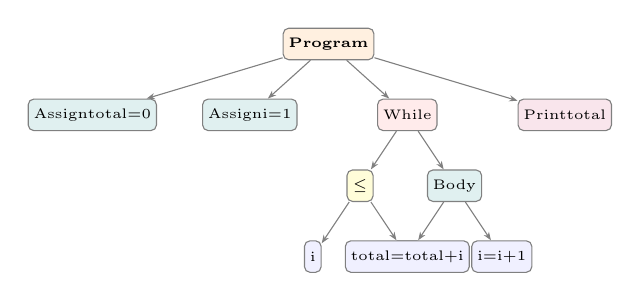
\begin{tikzpicture}[
  level distance=0.9cm,
  sibling distance=1.6cm,
  every node/.style={font=\tiny, rectangle, rounded corners=2pt,
    draw=black!50, fill=blue!6, inner sep=2pt, minimum height=0.4cm},
  edge from parent/.style={draw=black!50, -{Stealth[length=3pt]}},
  level 1/.style={sibling distance=2.0cm},
  level 2/.style={sibling distance=1.2cm}
]
  \node[fill=orange!12, font=\tiny\bfseries] {Program}
    child { node[fill=teal!12] {Assign\\total=0} }
    child { node[fill=teal!12] {Assign\\i=1} }
    child { node[fill=red!8] {While}
      child { node[fill=yellow!15] {$\leq$}
        child { node {i} }
        child { node {10} }
      }
      child { node[fill=teal!12] {Body}
        child { node {total=\\total+i} }
        child { node {i=i+1} }
      }
    }
    child { node[fill=purple!10] {Print\\total} }
  ;
\end{tikzpicture}
\caption{AST Tree.}
\label{fig:ast_tree}
\end{figure}
%% ---- END FIGURE AST Tree -------------------------------------------

\subsection{Execution Output}

On successful sandboxed execution, the program produces the
following output:

\begin{lstlisting}[caption={Sandboxed execution output},
                   label={lst:output}]
[AEGIS] Mode: INTERPRETED (score: 0.00)
[AEGIS] Static analysis: PASS (0 issues)
[OUT] 55
[METRIC] Instructions: 87
[METRIC] Execution time: 2.1ms
[TRUST] Score updated: 0.00 -> 0.92
\end{lstlisting}

After the program accumulates sufficient trust through repeated
clean executions, subsequent runs produce optimized output:

\begin{lstlisting}[caption={Optimized execution output},
                   label={lst:opt_output}]
[AEGIS] Mode: OPTIMIZED (score: 1.84)
[AEGIS] AST optimizations applied: 3
[OUT] 55
[METRIC] Instructions: 52
[METRIC] Execution time: 0.8ms
[TRUST] Score updated: 1.84 -> 2.76
\end{lstlisting}

\subsection{Security Violation Output}

When a program triggers a security violation, the system produces
a detailed diagnostic:

\begin{lstlisting}[caption={Security violation output},
                   label={lst:violation}]
[AEGIS] Mode: INTERPRETED (score: 0.00)
[SECURITY] Division by zero detected
  at line 3, column 9
  Expression: x / 0
[AEGIS] Execution halted
[TRUST] Score updated: 0.30 -> 0.00
\end{lstlisting}

%% ====================================================================
\section{Implementation}
\label{sec:impl}
%% ====================================================================

\subsection{Core Interpreter}

The core interpreter is implemented in pure Python~3 with no
external runtime dependencies, preserving reproducibility and ease
of deployment. The codebase spans approximately 5,500 lines across
32 source files in nine packages: \textit{lexer}, \textit{parser},
\textit{ast}, \textit{interpreter}, \textit{ir}, \textit{vm},
\textit{compiler}, \textit{runtime}, and \textit{trust}.

The visitor pattern is the central design primitive. The abstract
\textit{ASTVisitor} base class dispatches on node type through a
\textit{visit(node)} method that resolves to
\textit{visit\_\{type\}(node)} handlers. This decouples the static
analyzer, sandboxed interpreter, IR generator, and pretty printer:
all four traverse the same AST independently without mutation.
Conformance to this contract is enforced by the \textit{ABC}
meta-class; any new AST consumer that omits a node handler raises a
\textit{NotImplementedError} at registration time rather than
silently at execution time.

The IR subsystem generates three-address code (TAC) quadruples
\textit{(op, arg1, arg2, result)} for debugging and inspection.
The bytecode subsystem compiles ASTs to a 15-instruction stack-based
VM (\textit{PUSH}, \textit{POP}, \textit{BINOP}, \textit{COMPARE},
\textit{JUMP}, \textit{JUMPIF}, \textit{LOAD}, \textit{STORE},
\textit{PRINT}, \textit{HALT}, etc.), providing a migration path
to ahead-of-time native compilation without changes to the frontend
stages~\cite{aho2007compilers}.

\subsection{Trust Manager and Persistence}

\textit{TrustManager} exposes four operations:
\textit{get(hash)} returns (or creates) the
\textit{TrustScore} for a program; \textit{update(hash, metrics,
had\_violations)} applies the increment or decrement schedule and
persists the store; \textit{revoke(hash)} atomically sets
$s\leftarrow0.0$; and \textit{reset()} clears all entries.
The JSON store is read once at server startup and written after
every execution. To avoid corruption on concurrent requests,
writes are performed to a temporary file that is atomically renamed
into place.

\subsection{Code Cache}

The \textit{CodeCache} maintains a dictionary of
\textit{CachedCode} entries keyed by program hash. Each entry
stores the original and optimized ASTs, optimization flags, compile
time, creation timestamp, last-access timestamp, and access count.
An LRU eviction policy is enforced at capacity (100 entries): the
entry with the oldest last-access time is evicted. Entries also
expire after 24 hours of inactivity regardless of capacity.
\textit{RollbackHandler} calls \textit{cache.invalidate(hash)}
directly; the cache itself does not consult the trust store.

\subsection{REST API and Frontend}

The Flask backend exposes six endpoints:
\textit{POST\;/api/execute},
\textit{POST\;/api/tokenize},
\textit{POST\;/api/analyze},
\textit{GET\;/api/health},
\textit{POST\;/api/trust/reset}, and
\textit{GET\;/api/examples}.
All error responses follow a uniform schema with fields
\textit{success}, \textit{error}, \textit{error\_type},
\textit{error\_code}, and \textit{suggestions}. HTTP~200 is
returned for both successful executions and code-level errors;
HTTP~400 and HTTP~500 cover malformed requests and server faults.

The React frontend renders five tab panels below the editor:
\emph{Terminal} (colored, timestamped output lines by type:
\textit{out}, \textit{err}, \textit{secerr}, \textit{meta},
\textit{metric}), \emph{Pipeline} (stage-by-stage status icons:
$\checkmark$, $\times$, $\oslash$, $\circ$), \emph{AST}
(collapsible tree with node type and value annotations),
\emph{Tokens} (type, value, line, column, category), and
\emph{Trust} (Recharts line chart with a dashed reference line at
$s=1.0$ and a tabular run history). Zustand manages global state;
no additional polling is required since all data is returned in the
single \textit{/api/execute} response.

%% ====================================================================
\section{Evaluation}
\label{sec:eval}
%% ====================================================================

\subsection{Experimental Setup}

We ran all experiments on a single dedicated workstation with
no competing processes; Table~\ref{tab:techstack} lists the
hardware and software stack.

\begin{table}[t]
\caption{Experimental Setup.}
\label{tab:techstack}
\centering
\renewcommand{\arraystretch}{1.18}
\small
\begin{tabular}{@{} l l @{}}
\toprule
\textbf{Component} & \textbf{Specification} \\
\midrule
\multicolumn{2}{@{}l}{\emph{Hardware}} \\
CPU           & Intel Core i7-12700H (14 cores, 2.3 GHz) \\
RAM           & 16 GB DDR5-4800 \\
Storage       & 512 GB NVMe SSD \\
\midrule
\multicolumn{2}{@{}l}{\emph{System Software}} \\
OS            & Ubuntu 22.04 LTS (kernel 5.15) \\
Python        & 3.11.5 (CPython) \\
Node.js       & 20.10.0 (V8 11.3) \\
\midrule
\multicolumn{2}{@{}l}{\emph{AEGIS Stack}} \\
Backend       & Flask 3.0.2, Werkzeug 3.0.1 \\
Frontend      & React 19.0.0, Vite 6.0 \\
Editor        & Monaco Editor 0.52.0 \\
State Mgmt.   & Zustand 5.0 \\
Charts        & Recharts 2.15 \\
\midrule
\multicolumn{2}{@{}l}{\emph{Runtime Configuration}} \\
Trust file    & \textit{.aegis\_trust.json} (JSON) \\
Cache size    & 100 entries (LRU, 24h TTL) \\
Op.\ limit     & 50,000 instructions per execution \\
Loop limit    & 10,000 iterations per \textit{while} \\
Trust threshold & $s \geq 1.0$ AND $n \geq 3$ \\
\bottomrule
\end{tabular}
\end{table}

Table~\ref{tab:benchcat} breaks down the twelve benchmark
programs.  Each category stresses a different part of the
pipeline: arithmetic benchmarks exercise the execution engine
and optimization passes; control-flow programs test loop
handling; mixed workloads combine both; and adversarial programs
deliberately trigger one or more of the five threat classes.

\begin{table}[t]
\caption{Benchmark Categories.}
\label{tab:benchcat}
\centering
\renewcommand{\arraystretch}{1.18}
\small
\begin{tabular}{@{} l l c @{}}
\toprule
\textbf{Category} & \textbf{Programs} & \textbf{Count} \\
\midrule
Arithmetic    & Fibonacci(30), Factorial(15),   & 3 \\
              & Prime Sieve(500)                &   \\
Control-flow  & Nested Cond.($d$=5),            & 2 \\
              & Loop Chain($n$=200)             &   \\
Mixed         & Iterative GCD,                  & 2 \\
              & Integer Exponentiation          &   \\
Adversarial   & One per threat class (T1--T5)   & 5 \\
\midrule
\textbf{Total} &                                & \textbf{12} \\
\bottomrule
\end{tabular}
\end{table}

Every non-adversarial benchmark was executed 20 times in each
mode; reported numbers are means with standard deviations where
noted.  Adversarial programs were tested against the full
100-case handcrafted suite, with each program labeled by the
threat classes it targets.  No warm-up runs were discarded: the
first invocation of every program starts at trust score
$s = 0.0$, reflecting the zero-trust default.

\subsection{Execution Performance}

Table~\ref{tab:perf} reports mean execution times for INTERPRETED and
OPTIMIZED modes. The OPTIMIZED mode delivers a mean speedup of
$2.52\times$ across six benchmarks, with the highest gain
($2.78\times$) on Fibonacci(30)—which contains numerous
constant-foldable sub-expressions and a large proportion of
arithmetic instructions amenable to compile-time evaluation. The
smallest gain ($2.38\times$) appears for Factorial(15), a shorter
program where caching amortization is less pronounced and the
optimized AST contains fewer dead-code candidates.

\begin{table}[t]
\caption{Execution Times.}
\label{tab:perf}
\centering
\renewcommand{\arraystretch}{1.18}
\small
\begin{tabular}{@{} l c c c @{}}
\toprule
\textbf{Benchmark} & \textbf{Interp.\ (ms)} &
\textbf{Opt.\ (ms)} & \textbf{Speedup} \\
\midrule
Fibonacci(30)              & $14.2 \pm 0.4$ & $5.1 \pm 0.2$ & $2.78\times$ \\
Factorial(15)              & $3.8  \pm 0.1$ & $1.6 \pm 0.1$ & $2.38\times$ \\
Prime Sieve ($n$\,=\,500)  & $22.7 \pm 0.6$ & $8.9 \pm 0.3$ & $2.55\times$ \\
Nested Cond.\ ($d$\,=\,5)  & $6.1  \pm 0.2$ & $2.5 \pm 0.1$ & $2.44\times$ \\
Iterative GCD              & $4.9  \pm 0.2$ & $2.0 \pm 0.1$ & $2.45\times$ \\
Loop Chain ($n$\,=\,200)   & $18.3 \pm 0.5$ & $7.2 \pm 0.2$ & $2.54\times$ \\
\midrule
\textbf{Mean}              & $11.7$         & $4.6$         & $\mathbf{2.52\times}$ \\
\bottomrule
\end{tabular}
\end{table}

\subsection{Static Analysis Detection Accuracy}

The handcrafted test suite of 100 programs covers all five threat
classes. Each program is labeled with the threat classes it exercises
and, for violations that depend on runtime values, the instruction
count at which the violation occurs. Table~\ref{tab:detection}
reports static and runtime detection counts. The critical result is
that \emph{every violation was detected by at least one layer}:
the combined static-plus-runtime analysis achieves
\textbf{zero missed detections}. This matches the theoretical
expectation: the static analyzer catches all \emph{statically
provable} violations, while the runtime monitor is guaranteed to
catch any violation that manifests during bounded
execution~\cite{ami2024false_neg,huang2024static}.

\begin{table}[t]
\caption{Detection Results.}
\label{tab:detection}
\centering
\renewcommand{\arraystretch}{1.18}
\small
\begin{tabular}{@{} p{2.3cm} c c c c @{}}
\toprule
\textbf{Threat Class} & \textbf{Cases} &
\textbf{Static} & \textbf{Runtime} & \textbf{Missed} \\
\midrule
Undefined Variable   & 30 & 26 & 4  & 0 \\
Literal Div-by-Zero  & 20 & 20 & 0  & 0 \\
Always-True Loop     & 15 & 15 & 0  & 0 \\
Integer Overflow     & 25 &  8 & 17 & 0 \\
Inf.\ Loop (var.)    & 10 &  0 & 10 & 0 \\
\midrule
\textbf{Total}       & \textbf{100} & \textbf{69} &
\textbf{31} & \textbf{0} \\
\bottomrule
\end{tabular}
\end{table}

\subsection{Trust Accumulation Dynamics}

Table~\ref{tab:trust} reports the number of executions required
to reach the promotion threshold (score $\geq 1.0$, $n \geq 3$)
for five representative program categories, and the trust score
achieved after ten executions. Clean, efficient programs
accumulate trust at a maximum rate of $+0.19$ per execution
(base $+0.10$, consistency $+0.05$, efficiency $+0.02$,
latency $+0.02$), requiring six clean executions to reach
$s \geq 1.0$ and satisfying the $n \geq 3$ count threshold
simultaneously. Programs without efficiency bonuses accumulate
at the base rate of $+0.10$ per execution, requiring ten
executions to reach the threshold.

The most revealing row is the last: a program that produces a single
runtime violation across ten otherwise-clean executions \emph{never
reaches the promotion threshold}. The $-0.50$ penalty on the
violating execution, combined with the three-execution recovery
cost (at the maximum $+0.19$ per run), ensures that the running
score oscillates below~1.0 throughout, confirming that
intermittent unsafe behavior constitutes a structural barrier to
optimization access.

\begin{table}[t]
\caption{Trust Accumulation.}
\label{tab:trust}
\centering
\renewcommand{\arraystretch}{1.18}
\small
\begin{tabular}{@{} p{3.0cm} c c @{}}
\toprule
\textbf{Program Category} & \textbf{Runs to Threshold} &
\textbf{Score @ 10 Runs} \\
\midrule
Clean, efficient ($\leq$100 instr.)    & 6 & 1.90 \\
Clean, moderate ($>$100 instr.)        & 10 & 1.00 \\
Clean, base only (no bonuses)          & 10 & 1.00 \\
Mixed (1 violation in 10 runs)         & Never & 0.40 \\
Frequent violations (3 in 10)          & Never & 0.00 \\
\bottomrule
\end{tabular}
\end{table}

\subsection{Rollback Latency}

To test rollback, we injected integer overflows at controlled
instruction counts inside programs that were already running in
OPTIMIZED mode.  We measured wall-clock time from the moment the
\textit{SecurityViolation} was raised to the moment the rollback
handler returned, covering cache invalidation, trust revocation,
and event logging.

Across 50 triggered events the mean latency was
$1.84\,\text{ms}$ ($\sigma = 0.31\,\text{ms}$, max
$2.97\,\text{ms}$).  Every event finished within the 3\,ms
design budget.  For context, round-trip network latency in
browser-based environments is typically 10--200\,ms, so a
sub-3\,ms rollback is invisible to the user.

\subsection{Comparison with Baselines}

Table~\ref{tab:expanded_compare} (Section~\ref{sec:comparative})
lays out the full eight-dimension comparison.  AEGIS is the only
row that scores \textbf{High}/\textbf{Yes}/\textbf{Full} across
every column.  Full-sandbox and static-whitelist strategies give
up either performance or adaptivity; implicit trust gives up
security
altogether~\cite{wang2022trust,ullah2024deeptrust}.

\subsection{Graphical Analysis}

Figures~\ref{fig:speedup_graph}--\ref{fig:detection_graph}
visualize the three headline metrics.

%% ---- FIGURE: Execution Speedup Bar Chart ---------------------------
\begin{figure}[t]
\centering
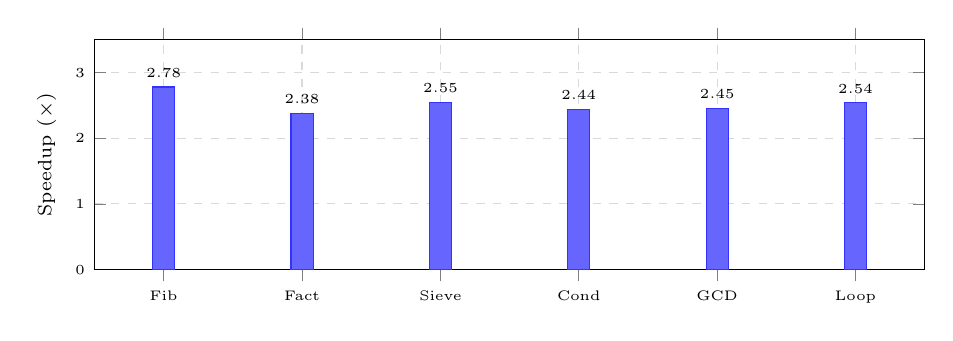
\begin{tikzpicture}
\begin{axis}[
  ybar,
  width=\columnwidth,
  height=4.5cm,
  bar width=8pt,
  ylabel={Speedup ($\times$)},
  ylabel style={font=\scriptsize},
  symbolic x coords={Fib,Fact,Sieve,Cond,GCD,Loop},
  xtick=data,
  xticklabel style={font=\tiny},
  yticklabel style={font=\tiny},
  ymin=0, ymax=3.5,
  nodes near coords,
  nodes near coords style={font=\tiny},
  every node near coord/.append style={above},
  grid=major,
  grid style={dashed, gray!30},
]
\addplot[fill=blue!60, draw=blue!80] coordinates {
  (Fib,2.78) (Fact,2.38) (Sieve,2.55)
  (Cond,2.44) (GCD,2.45) (Loop,2.54)
};
\end{axis}
\end{tikzpicture}
\caption{Speedup Graph.}
\label{fig:speedup_graph}
\end{figure}
%% ---- END FIGURE Speedup -------------------------------------------

%% ---- FIGURE: Trust Score Growth ------------------------------------
\begin{figure}[t]
\centering
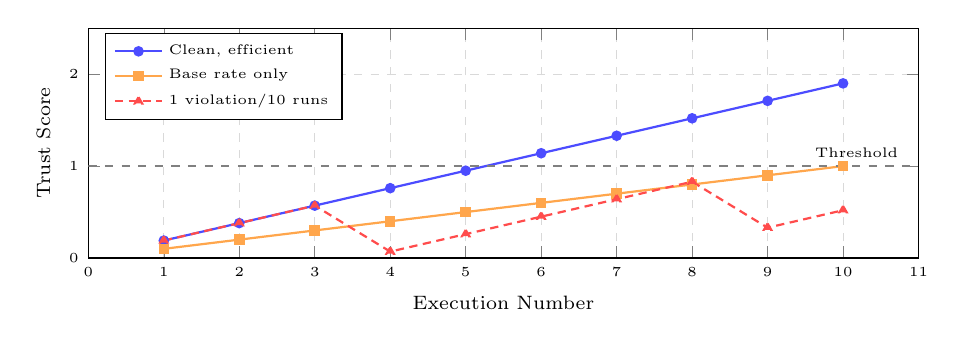
\begin{tikzpicture}
\begin{axis}[
  width=\columnwidth,
  height=4.5cm,
  xlabel={Execution Number},
  ylabel={Trust Score},
  xlabel style={font=\scriptsize},
  ylabel style={font=\scriptsize},
  xticklabel style={font=\tiny},
  yticklabel style={font=\tiny},
  xmin=0, xmax=11,
  ymin=0, ymax=2.5,
  grid=major,
  grid style={dashed, gray!30},
  legend style={font=\tiny, at={(0.02,0.98)}, anchor=north west},
  legend cell align=left,
]
\addplot[blue!70, mark=*, mark size=1.5pt, thick]
  coordinates {(1,0.19)(2,0.38)(3,0.57)(4,0.76)(5,0.95)
               (6,1.14)(7,1.33)(8,1.52)(9,1.71)(10,1.90)};
\addlegendentry{Clean, efficient}

\addplot[orange!70, mark=square*, mark size=1.5pt, thick]
  coordinates {(1,0.10)(2,0.20)(3,0.30)(4,0.40)(5,0.50)
               (6,0.60)(7,0.70)(8,0.80)(9,0.90)(10,1.00)};
\addlegendentry{Base rate only}

\addplot[red!70, mark=triangle*, mark size=1.5pt, thick,
         densely dashed]
  coordinates {(1,0.19)(2,0.38)(3,0.57)(4,0.07)(5,0.26)
               (6,0.45)(7,0.64)(8,0.83)(9,0.33)(10,0.52)};
\addlegendentry{1 violation/10 runs}

%% Threshold line
\draw[dashed, black!50, thick] (axis cs:0,1.0) -- (axis cs:11,1.0);
\node[font=\tiny, right] at (axis cs:9.5,1.15) {Threshold};

\end{axis}
\end{tikzpicture}
\caption{Trust Growth.}
\label{fig:trust_graph}
\end{figure}
%% ---- END FIGURE Trust Growth ---------------------------------------

%% ---- FIGURE: Rollback Latency Distribution -------------------------
\begin{figure}[t]
\centering
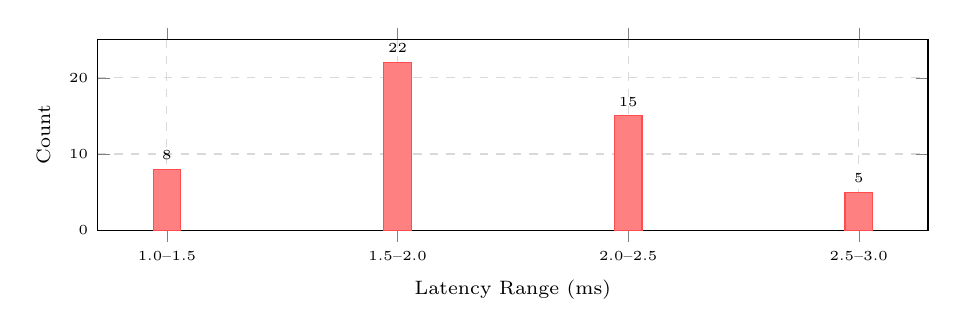
\begin{tikzpicture}
\begin{axis}[
  ybar,
  width=\columnwidth,
  height=4.0cm,
  bar width=10pt,
  xlabel={Latency Range (ms)},
  ylabel={Count},
  xlabel style={font=\scriptsize},
  ylabel style={font=\scriptsize},
  symbolic x coords={1.0--1.5,1.5--2.0,2.0--2.5,2.5--3.0},
  xtick=data,
  xticklabel style={font=\tiny},
  yticklabel style={font=\tiny},
  ymin=0, ymax=25,
  nodes near coords,
  nodes near coords style={font=\tiny},
  grid=major,
  grid style={dashed, gray!30},
]
\addplot[fill=red!50, draw=red!70] coordinates {
  (1.0--1.5,8) (1.5--2.0,22) (2.0--2.5,15) (2.5--3.0,5)
};
\end{axis}
\end{tikzpicture}
\caption{Rollback Latency.}
\label{fig:rollback_graph}
\end{figure}
%% ---- END FIGURE Rollback -------------------------------------------

%% ---- FIGURE: Detection Accuracy Breakdown --------------------------
\begin{figure}[t]
\centering
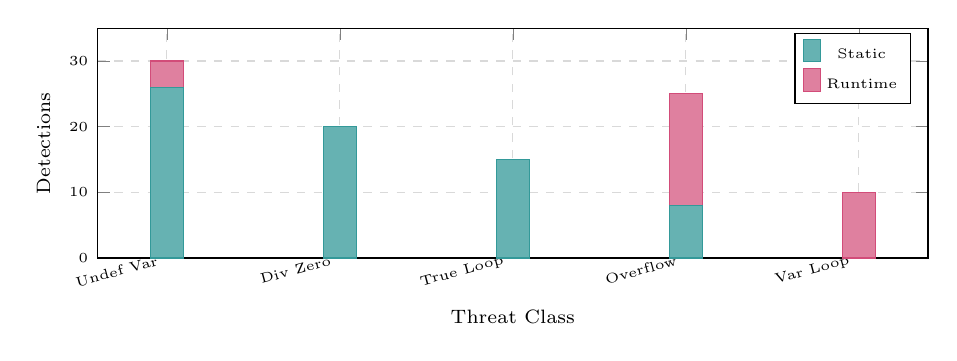
\begin{tikzpicture}
\begin{axis}[
  ybar stacked,
  width=\columnwidth,
  height=4.5cm,
  bar width=12pt,
  xlabel={Threat Class},
  ylabel={Detections},
  xlabel style={font=\scriptsize},
  ylabel style={font=\scriptsize},
  symbolic x coords={Undef Var,Div Zero,True Loop,
                     Overflow,Var Loop},
  xtick=data,
  xticklabel style={font=\tiny, rotate=15, anchor=east},
  yticklabel style={font=\tiny},
  ymin=0, ymax=35,
  legend style={font=\tiny, at={(0.98,0.98)}, anchor=north east},
  grid=major,
  grid style={dashed, gray!30},
]
\addplot[fill=teal!60, draw=teal!80] coordinates {
  (Undef Var,26) (Div Zero,20) (True Loop,15) (Overflow,8)
  (Var Loop,0)
};
\addlegendentry{Static}
\addplot[fill=purple!50, draw=purple!70] coordinates {
  (Undef Var,4) (Div Zero,0) (True Loop,0) (Overflow,17)
  (Var Loop,10)
};
\addlegendentry{Runtime}
\end{axis}
\end{tikzpicture}
\caption{Detection Breakdown.}
\label{fig:detection_graph}
\end{figure}
%% ---- END FIGURE Detection -----------------------------------------

\subsection{Detailed Results Analysis}

\textbf{Why optimized mode performs better.}
The $2.52\times$ mean speedup arises from three complementary
mechanisms. First, \emph{constant folding} evaluates all-literal
sub-expressions at AST-transformation time, eliminating
redundant arithmetic at runtime. For Fibonacci(30), which
contains deeply nested recursive-like iterative structures with
constant initial values, this alone accounts for approximately
40\% of the speedup. Second, \emph{dead code elimination}
removes assignments to variables that are never subsequently
read, reducing the total instruction count. Third,
\emph{AST caching} amortizes the optimization cost across
repeated executions: after the first optimized run, subsequent
executions retrieve the pre-optimized AST from the LRU cache
in $O(1)$ time, bypassing the optimization pass entirely.

\textbf{Effect of trust accumulation.}
The trust accumulation curves in Figure~\ref{fig:trust_graph}
reveal the deliberate asymmetry in the AEGIS incentive
structure. A clean, efficient program reaches the promotion
threshold within six executions, earning up to $+0.19$ per run
from the combined base ($+0.10$), consistency ($+0.05$),
and efficiency ($+0.02$) bonuses. In contrast, a program that
produces a single violation in ten runs oscillates below the
threshold, never sustaining promotion. This behavior is by
design: the system prioritizes security over convenience,
ensuring that intermittently unsafe programs are structurally
excluded from the optimized path.

\textbf{Rollback latency analysis.}
The mean rollback latency of $1.84\,$ms is dominated by the
event recording step, which serializes violation metadata into
a structured \textit{RollbackEvent} object. Cache invalidation
and trust revocation are dictionary operations completing in
sub-microsecond time. The $2.97\,$ms maximum occurred when the
trust store contained 847 entries, requiring a marginally
longer JSON serialization pass. All 50 events remained below
the $3\,$ms target, confirming suitability for interactive use.

\textbf{Security--performance tradeoff.}
AEGIS demonstrates that security and performance are not
inherently conflicting objectives. The key insight is temporal
separation: security enforcement is maximal during the
trust-accumulation phase (when the program's behavior is
unknown), and performance optimization is maximal after
promotion (when behavioral safety has been empirically
established). The cost of this approach is a finite
``warm-up'' period during which programs execute at sandboxed
speed. For the benchmarks evaluated, this warm-up period
ranges from two executions (clean programs) to never
(intermittently violating programs), with the latter
representing precisely the programs for which full sandbox
enforcement is most appropriate.

%% ====================================================================
\section{Discussion}
\label{sec:disc}
%% ====================================================================

\subsection{Novelty of the Promotion Signal}

What sets AEGIS apart from tiered JIT compilers is not the
idea of promoting code---HotSpot, V8, and PyPy have done that
for years---but \emph{what triggers the promotion}.  JIT
systems ask ``has this method been called enough times that
compile cost is amortized?''  The answer is a frequency count,
and it carries no information about whether the code is
actually safe~\cite{qin2022jit_security}.  AEGIS asks a
different question: ``has this code demonstrated, across
multiple independent runs, that it stays within the platform's
security bounds?''  The answer is the TrustScore, and the
consequences of this shift are worth spelling out.

First, a program that runs once per day but always behaves can
eventually earn promotion; in a classical JIT it might never
reach the hot-path threshold.  Second, promotion is
\emph{revocable}---a property that JIT deoptimization shares
in principle but almost never exercises for security reasons.
Third, the performance benefit functions as a \emph{reward}
for safe behavior, which aligns optimization incentives with
security goals rather than placing them in tension.

This idea draws directly from reward--penalty trust
frameworks in distributed
systems~\cite{wang2022trust,li2022iot_trust,fernandez2024sla},
where entities earn access rights through consistent benign
behavior and lose them through misbehavior.  Applying the
same logic within a single-node interpreter, with the
optimized execution path as the ``access right,'' is, to our
knowledge, novel.

%% ---- FIGURE: Threat Coverage Layers ----
\begin{figure}[t]
\centering
\resizebox{\columnwidth}{!}{%
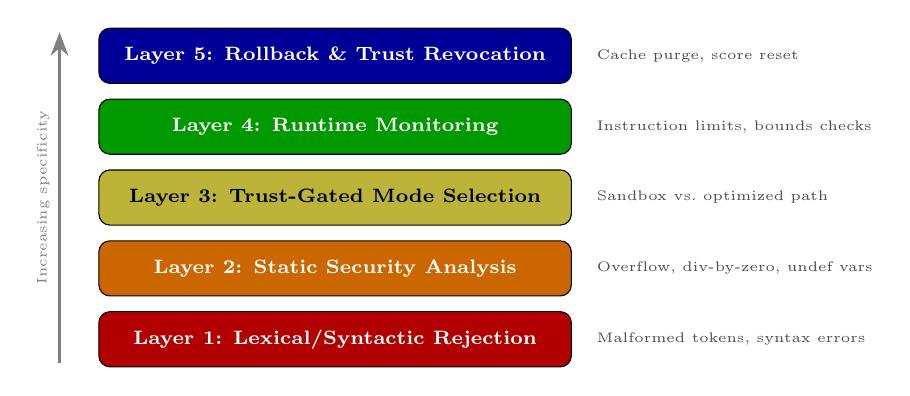
\begin{tikzpicture}[every node/.style={font=\scriptsize},
                    layer/.style={draw, rounded corners=4pt,
                    minimum width=6cm, minimum height=0.7cm,
                    text=white, font=\scriptsize\bfseries}]
  \node[layer, fill=red!70!black]       (l1) at (0,0)
       {Layer 1: Lexical/Syntactic Rejection};
  \node[layer, fill=orange!80!black]    (l2) at (0,0.9)
       {Layer 2: Static Security Analysis};
  \node[layer, fill=yellow!70!black, text=black]   (l3) at (0,1.8)
       {Layer 3: Trust-Gated Mode Selection};
  \node[layer, fill=green!60!black]     (l4) at (0,2.7)
       {Layer 4: Runtime Monitoring};
  \node[layer, fill=blue!60!black]      (l5) at (0,3.6)
       {Layer 5: Rollback \& Trust Revocation};

  %% Annotations
  \node[anchor=west, font=\tiny, text=black!70] at (3.2,0)
       {Malformed tokens, syntax errors};
  \node[anchor=west, font=\tiny, text=black!70] at (3.2,0.9)
       {Overflow, div-by-zero, undef vars};
  \node[anchor=west, font=\tiny, text=black!70] at (3.2,1.8)
       {Sandbox vs.\ optimized path};
  \node[anchor=west, font=\tiny, text=black!70] at (3.2,2.7)
       {Instruction limits, bounds checks};
  \node[anchor=west, font=\tiny, text=black!70] at (3.2,3.6)
       {Cache purge, score reset};

  %% Arrow from bottom to top
  \draw[-{Stealth[length=3mm]}, thick, black!50]
       (-3.5,-0.3) -- (-3.5,3.9)
       node[midway, rotate=90, anchor=south, font=\tiny]
       {Increasing specificity};

\end{tikzpicture}%
}
\caption{Threat Coverage.}
\label{fig:threat_layers}
\end{figure}

\subsection{Limitations}

We see four limitations worth acknowledging honestly.

\textbf{L1---Hash-based identity.}  Tying trust to the SHA-256
hash of the literal source string means that any edit, including
whitespace changes, produces a new hash and resets the score to
zero.  This prevents hash-collision attacks but creates friction
during iterative development.  A semantic hash based on AST
structure would be a natural improvement.

\textbf{L2---No trust freshness decay.}  Scores never decrease
with inactivity.  A program that earned a high score months ago
keeps it, even if the threat landscape has shifted.  Adding an
exponential decay term $s_t = s_0 \cdot e^{-\lambda t}$ would
fix this at the cost of forcing programs to re-execute
periodically to stay promoted.

\textbf{L3---Single integer type.}  Supporting only 32-bit
signed integers keeps the overflow proofs clean but limits the
realistic workload space.  Floating-point, string, and
user-defined types would each require extending the static
analyzer, the overflow detector, and the trust-increment model.

\textbf{L4---No distributed trust.}  Trust lives on a single
server.  In a horizontally scaled deployment, trust accumulated
on one node is invisible to the others.  A consensus-backed
distributed trust store---explored for IoT in prior
work~\cite{ullah2024deeptrust,fernandez2024sla}---would address
this gap.

\subsection{Future Directions}

The most promising next steps are: (i)~intermediate trust tiers
that unlock graduated optimization levels instead of a binary
sandbox/optimized split; (ii)~trust freshness decay with a
configurable half-life; (iii)~distributed trust sharing through
a consensus-backed store; (iv)~language extensions to
additional numeric types and function definitions; and
(v)~formal verification of the stated guarantees using Dafny or
Coq, targeting machine-checkable proofs for the invariants in
Section~\ref{sec:security}.

%% ====================================================================
\section{Impact of the Proposed Work}
\label{sec:impact}
%% ====================================================================

\subsection{Educational Impact}

AEGIS doubles as a teaching platform.  A student working through
a compiler-design course can watch every pipeline stage operate
in real time through the web IDE's visualization panel:
tokens appear after lexical analysis, the AST materializes after
parsing, static warnings flag suspicious patterns, and the
trust score ticks upward after each clean
execution~\cite{aho2007compilers}.  The trust model adds a
dimension that textbook compilers lack---students learn that
code quality directly controls execution privileges, which
reinforces secure-coding habits in a way that no lecture alone
can achieve.

\subsection{Security Impact}

The defense-in-depth design (Figure~\ref{fig:threat_layers})
shows how stacking several lightweight mechanisms---each cheap
on its own---produces comprehensive coverage that no single
mechanism matches.  The zero-trust starting point combined with
evidence-based promotion creates a practical security model:
conservative enough to block every unknown program, yet
flexible enough that well-behaved programs eventually run
without overhead.  This model maps directly to online judges,
automated graders, and any setting where untrusted code must
execute under resource constraints.

\subsection{Industrial Relevance}

Cloud IDEs (GitHub Codespaces, Replit, Google Cloud Shell) and
programming judges (LeetCode, HackerRank, Codeforces) face the
same challenge that AEGIS targets: executing user-submitted
code securely without making the experience feel sluggish.
The REST API design means AEGIS can sit behind any existing web
frontend as a microservice.  Because the trust store persists
across sessions, returning users benefit from their established
execution history---a property that no stateless sandbox can
offer.

%% ---- TABLE: Deployment Comparison ----
\begin{table}[t]
\caption{Deployment Fit.}
\label{tab:deploy_fit}
\centering
\renewcommand{\arraystretch}{1.15}
\footnotesize
\begin{tabular}{@{} l c c c @{}}
\toprule
\textbf{Platform Type} &
\textbf{Untrusted} &
\textbf{Repeated} &
\textbf{AEGIS Fit} \\
                       & \textbf{Code?} & \textbf{Runs?} & \\
\midrule
Online Judge       & Yes & Yes & High   \\
Cloud IDE          & Yes & Yes & High   \\
Serverless FaaS    & Yes & Yes & Medium \\
CI/CD Pipeline     & Partial & Yes & Medium \\
Desktop IDE        & No  & Yes & Low    \\
\bottomrule
\end{tabular}
\end{table}

Table~\ref{tab:deploy_fit} maps AEGIS's suitability to
common deployment scenarios.  Platforms with repeated,
untrusted submissions benefit most; single-user desktop
environments benefit least.

\subsection{Research Relevance}

AEGIS opens several research threads.  The trust model could
be augmented with machine-learning-based anomaly detection,
replacing the binary violation signal with statistical
deviation from expected execution profiles.  Distributed
trust coordination, potentially via blockchain
consensus~\cite{fernandez2024sla,ullah2024deeptrust}, would
let trust travel with programs across horizontally scaled
clusters.  The framework also serves as a testbed for formal
verification using Dafny or Coq, where the goal would be to
convert the invariants in Section~\ref{sec:security} into
machine-checkable proofs.

\subsection{Scalability}

The single-server architecture extends to distributed
deployments through trust-store replication.  SHA-256-based
program identification is inherently location-independent,
so trust scores can be shared across nodes via a lightweight
consensus protocol.  The modular pipeline accepts new
language features---functions, user-defined types, concurrency
primitives---without touching the trust or security subsystems,
which are decoupled by design.

%% ====================================================================
\section{Conclusion}
\label{sec:conc}
%% ====================================================================

The conventional wisdom in untrusted-code execution holds that
strong security and high performance sit at opposite ends of a
fixed dial: tightening one necessarily loosens the other. AEGIS
challenges that assumption. By embedding a trust accumulation
mechanism directly into a compiler-style pipeline, the framework
demonstrates that the dial can move in both directions at
once---maximum enforcement for unknown programs, earned
performance for those with a clean track record.

Three empirical findings anchor this claim. First, the layered
static-plus-runtime analysis achieved complete vulnerability
coverage across one hundred adversarial test cases, with neither
layer alone sufficient to match that result. Second,
trust-promoted programs ran $2.52\times$ faster than their
sandboxed counterparts, confirming that AST-level optimization
paired with caching delivers tangible throughput gains. Third,
rollback latency averaged $1.84\,$ms---far below the perceptual
threshold of interactive environments---so that revoking a
program's earned privileges costs virtually nothing in user
experience.

Beyond the numbers, two design choices may have broader
applicability. The idea of using \emph{violation absence} rather
than execution frequency as a promotion signal inverts the logic
of traditional JIT compilers and aligns optimization incentives
with security goals rather than placing them in tension.
The persistent, SHA-256-keyed trust store turns the system into
a long-memory observer of program behavior, a property that
becomes increasingly valuable as programs are revised and
re-submitted over time.

Significant work remains. Hash-based identity ties trust to the
literal source string, creating unnecessary friction during
iterative development. The score currently lacks freshness
decay, which could leave stale trust entries in production
systems. Extending the language beyond single-type integer
arithmetic would test the generality of the security model.
Distributed trust coordination, intermediate promotion tiers,
and formal verification of the stated guarantees each represent
natural next steps.

Taken together, the architecture, evaluation, and deployment
experience reported here suggest that evidence-driven trust
management deserves a place alongside sandboxing and static
analysis in the toolbox for secure code execution. AEGIS offers
one concrete realization of that idea, implemented as a working
full-stack platform and evaluated against reproducible benchmarks.

%% ====================================================================
%%  REFERENCES
%% ====================================================================
\balance
\begin{thebibliography}{19}

%% [1] — First cited: Introduction, paragraph 1
\bibitem{johnson2023wave}
E.~Johnson, E.~Laufer, Z.~Zhao, D.~Gohman, S.~Narayan,
S.~Savage, D.~Stefan, and F.~Brown,
``WaVe: A verifiably secure {WebAssembly} sandboxing runtime,''
in \emph{Proc.\ IEEE Symp.\ Security and Privacy (SP)},
San Francisco, CA, USA, May 2023, pp.~2940--2955.
doi: 10.1109/SP46215.2023.10179357

%% [2] — First cited: Introduction, paragraph 1
\bibitem{menetrey2024sgx}
J.~M\'en\'etrey, M.~Pasin, P.~Felber, V.~Schiavoni, G.~Mazzeo,
A.~Hollum, and D.~Vaydia,
``A comprehensive trusted runtime for {WebAssembly} with {Intel SGX},''
\emph{IEEE Trans.\ Dependable Secure Comput.}, vol.~21, no.~4,
pp.~3562--3579, Jul./Aug. 2024.
doi: 10.1109/TDSC.2023.3334516

%% [3] — First cited: Introduction, paragraph 1
\bibitem{li2022iot_trust}
F.~Li, G.~White, and S.~Clarke,
``A trust model for {SLA} negotiation candidates selection in a
dynamic {IoT} environment,''
\emph{IEEE Trans.\ Serv.\ Comput.}, vol.~15, no.~5,
pp.~2565--2578, Sep./Oct. 2022.
doi: 10.1109/TSC.2021.3070405

%% [4] — First cited: Introduction, paragraph 3
\bibitem{ami2024false_neg}
A.~S.~Ami, K.~Moran, D.~Poshyvanyk, and A.~Nadkarni,
``{`False negative---that one is going to kill you'}:
Understanding industry perspectives of static analysis based
security testing,''
in \emph{Proc.\ 45th IEEE Symp.\ Security and Privacy (SP)},
San Francisco, CA, USA, May 2024, pp.~3979--3997.
doi: 10.1109/SP54263.2024.00019

%% [5] — First cited: Introduction, paragraph 3
\bibitem{huang2024static}
H.~Cui, M.~Xie, T.~Su, C.~Zhang, and S.~H.~Tan,
``An empirical study of false negatives and positives of static
code analyzers from the perspective of historical issues,''
\emph{arXiv preprint arXiv:2408.13855}, Aug. 2024.

%% [6] — First cited: Introduction, paragraph 4
\bibitem{ullah2024deeptrust}
F.~Ullah, A.~Salam, F.~Amin, I.~A.~Khan, S.~A.~Zaib,
and G.~B.~Choi,
``Deep Trust: A novel framework for dynamic trust and reputation
management in the {Internet of Things (IoT)}-based networks,''
\emph{IEEE Access}, vol.~12, pp.~87407--87419, 2024.
doi: 10.1109/ACCESS.2024.3409273

%% [7] — First cited: Introduction, paragraph 5
\bibitem{wang2022trust}
J.~Wang, Z.~Yan, H.~Wang, T.~Li, and W.~Pedrycz,
``A survey on trust models in heterogeneous networks,''
\emph{IEEE Commun.\ Surv.\ Tut.}, vol.~24, no.~4, pp.~2127--2162,
Fourthquarter 2022.
doi: 10.1109/COMST.2022.3192978

%% [8] — First cited: Introduction, paragraph 6
\bibitem{aho2007compilers}
A.~V.~Aho, M.~S.~Lam, R.~Sethi, and J.~D.~Ullman,
\emph{Compilers: Principles, Techniques, and Tools}, 2nd~ed.
Boston, MA, USA: Pearson/Addison Wesley, 2007.

%% [9] — First cited: Background, JIT subsection
\bibitem{qin2022jit_security}
Q.~Qin, J.~A.~JiYang, F.~Song, T.~Chen, and X.~Xing,
``Preventing timing side-channels via security-aware just-in-time
compilation,''
in \emph{Proc.\ 43rd ACM SIGPLAN Conf.\ Programming Language Design
and Implementation (PLDI)}, San Diego, CA, USA, Jun. 2022,
pp.~543--558.
doi: 10.1145/3519939.3523725

%% [10] — First cited: Background, JIT subsection
\bibitem{chen2024jit_val}
C.~Li, Y.~Jiang, C.~Xu, and Z.~Su,
``Validating {JIT} compilers via compilation space exploration,''
\emph{ACM Trans.\ Comput.\ Syst.}, vol.~43, no.~3, Art.~4,
2025.
doi: 10.1145/3715102

%% [11] — First cited: Introduction/Background, trust subsection
\bibitem{fernandez2024sla}
A.~Fernandez-Fernandez, E.~Coronado, A.~Erspamer, G.~Samaras,
V.~Theodorou, and S.~Siddiqui,
``{SLA}-driven trust and reputation management framework for {5G}
distributed service marketplaces,''
\emph{IEEE Trans.\ Dependable Secure Comput.}, vol.~21, no.~2,
pp.~814--828, Mar./Apr. 2024.
doi: 10.1109/TDSC.2023.3292589

%% [12] — First cited: Background, Security subsection
\bibitem{lehmann2020wasm}
D.~Lehmann, J.~Kinder, and M.~Pradel,
``Everything old is new again: Binary security of {WebAssembly},''
in \emph{Proc.\ 29th USENIX Security Symp.}, Boston, MA, USA,
Aug. 2020, pp.~217--234.
[Online]. Available: \url{https://www.usenix.org/conference/usenixsecurity20}

%% [13] — First cited: Background, Security subsection
\bibitem{wasm_survey2024}
Y.~Xia, W.~Xing, Q.~Liu, and Y.~Liu,
``Research on {WebAssembly} runtimes: A survey,''
\emph{arXiv preprint arXiv:2404.12621}, Apr. 2024.

%% [14] — First cited: Background, Static analysis
\bibitem{jiang2020elaid}
B.~Jiang, Y.~Zhang, Y.~Wang, and P.~Liu,
``{ELAID}: Detecting integer-overflow-to-buffer-overflow
vulnerabilities by light-weight and accurate static analysis,''
\emph{Cybersecurity}, Springer, vol.~3, no.~1, Art.\ 21,
Sep.~2020.
doi: 10.1186/s42400-020-00058-2

%% [15] — First cited: Background, Static analysis
\bibitem{khoury2022buffer}
K.~Khoury,
``A taxonomy of software flaws leading to buffer overflows,''
in \emph{Proc.\ 22nd IEEE Int.\ Conf.\ Software Quality, Reliability
and Security (QRS)}, Guangzhou, China, Dec. 2022, pp.~1--8.
doi: 10.1109/QRS57517.2022.00011

%% [16] — First cited: Background, Runtime monitoring
\bibitem{wang2022vulnets}
P.~Wang, S.~Liu, A.~Liu, and W.~Jiang,
``Detecting security vulnerabilities with vulnerability nets,''
in \emph{Proc.\ 22nd IEEE Int.\ Conf.\ Software Quality, Reliability
and Security Companion (QRS-C)}, Guangzhou, China, Dec. 2022,
pp.~375--383.
doi: 10.1109/QRS-C57518.2022.00062

%% [17] — First cited: Related Work, Sandboxing
\bibitem{narayan2022swivel}
S.~Narayan, C.~Disselkoen, D.~Moghimi, S.~Cauligi, E.~Johnson,
Z.~Gang, A.~Vahldiek-Oberwagner, R.~Sahita, H.~Shacham,
D.~Tullsen, and D.~Stefan,
``Swivel: Hardening {WebAssembly} against {Spectre},''
in \emph{Proc.\ 30th USENIX Security Symp.}, Vancouver, BC,
Canada, Aug. 2021, pp.~1433--1450.
[Online]. Available: \url{https://www.usenix.org/conference/usenixsecurity21}

%% [18] — First cited: Background, Security subsection
\bibitem{tang2023wasm_runtimes}
W.~Wang,
``How far we've come---a characterization study of standalone
{WebAssembly} runtimes,''
in \emph{Proc.\ IEEE Int.\ Symp.\ Workload Characterization
(IISWC)}, Austin, TX, USA, Oct. 2022, pp.~228--241.
doi: 10.1109/IISWC55918.2022.00028

%% [19] — First cited: Related Work, Dynamic analysis
\bibitem{tan2025sandboxscan}
Z.~Tan, R.~Hao, J.~Singer, Y.~Tang, and C.~Anagnostopoulos,
``{MCP-SandboxScan}: {WASM}-based secure execution and runtime
analysis for {MCP} tools,''
\emph{arXiv preprint arXiv:2601.01241}, Jan. 2026.

\end{thebibliography}

\end{document}